%Carattere dimensione 12
\documentclass[12pt]{report}

%Margini e interlinea
\usepackage[top=2.5cm, bottom=2.5cm, left=4cm, right=2.5cm, centering]{geometry}
\linespread{1.5}

%Librerie utili
\usepackage[italian]{babel}
\usepackage[utf8]{inputenc}
\usepackage{mathptmx} % font times new roman (simile)
\usepackage{graphicx}
\usepackage{titlesec} % per la formattazione dei titoli delle sezioni, capitoli etc.
\usepackage{float} % per il posizionamento di immagini
\usepackage{titlesec} % per i titoli
\usepackage{listings} % per il codice di programmazione
\renewcommand{\lstlistingname}{Codice}% Listing -> Codice
\usepackage{xcolor}  % stile del codice

\definecolor{mygreen}{rgb}{0,0.6,0}
\definecolor{mygray}{rgb}{0.5,0.5,0.5}
\definecolor{mymauve}{rgb}{0.58,0,0.82}
\definecolor{darkgray}{rgb}{.4,.4,.4}
\definecolor{navy}{HTML}{000080}
\definecolor{purple}{rgb}{0.65, 0.12, 0.82}
\definecolor{codepurple}{rgb}{0.58,0,0.82}
\definecolor{backcolour}{rgb}{0.95,0.95,0.92}

%Customize a bit the look
\lstset{ %
belowcaptionskip=0.5em,
backgroundcolor=\color{backcolour}, % choose the background color; you must add \usepackage{color} or \usepackage{xcolor}
basicstyle=\footnotesize, % the size of the fonts that are used for the code
breakatwhitespace=false, % sets if automatic breaks should only happen at whitespace
breaklines=true, % sets automatic line breaking
captionpos=b, % sets the caption-position to bottom
commentstyle=\color{mygreen}, % comment style
deletekeywords={...}, % if you want to delete keywords from the given language
escapeinside={\%*}{*)}, % if you want to add LaTeX within your code
extendedchars=true, % lets you use non-ASCII characters; for 8-bits encodings only, does not work with UTF-8
frame=single, % adds a frame around the code
keepspaces=true, % keeps spaces in text, useful for keeping indentation of code (possibly needs columns=flexible)
keywordstyle=\color{codepurple}, % keyword style
% language=Octave, % the language of the code
morekeywords={*,...}, % if you want to add more keywords to the set
numbers=left, % where to put the line-numbers; possible values are (none, left, right)
numbersep=5pt, % how far the line-numbers are from the code
numberstyle=\tiny\color{mygray}, % the style that is used for the line-numbers
rulecolor=\color{black}, % if not set, the frame-color may be changed on line-breaks within not-black text (e.g. comments (green here))
showspaces=false, % show spaces everywhere adding particular underscores; it overrides 'showstringspaces'
showstringspaces=false, % underline spaces within strings only
showtabs=false, % show tabs within strings adding particular underscores
stepnumber=1, % the step between two line-numbers. If it's 1, each line will be numbered
stringstyle=\color{mymauve}, % string literal style
tabsize=2, % sets default tabsize to 2 spaces
title=\lstname % show the filename of files included with \lstinputlisting; also try caption instead of title
}
%END of listing package%
 
%define Javascript language
\lstdefinelanguage{JavaScript}{
keywords={typeof, new, true, false, catch, function, return, null, catch, switch, var, if, in, while, do, else, case, break},
keywordstyle=\color{blue}\bfseries,
ndkeywords={class, export, boolean, throw, implements, import, this, constructor},
ndkeywordstyle=\color{navy}\bfseries,
identifierstyle=\color{black},
sensitive=false,
comment=[l]{//},
morecomment=[s]{/*}{*/},
commentstyle=\color{mygreen}\ttfamily,
stringstyle=\color{red}\ttfamily,
morestring=[b]',
morestring=[b]"
}
 
\lstset{
language=JavaScript,
extendedchars=true,
basicstyle=\footnotesize\ttfamily,
showstringspaces=false,
showspaces=false,
numbers=left,
numberstyle=\footnotesize,
numbersep=9pt,
tabsize=2,
breaklines=true,
showtabs=false,
captionpos=b
}

\titleformat{\chapter}[block]
  {\normalfont\LARGE\bfseries}{\thechapter.}{0.5em}{\LARGE}
\titlespacing*{\chapter}{0pt}{-20pt}{25pt}

\usepackage{blindtext} % per lorem ipsum 
\usepackage{csquotes}

\usepackage[backend=biber, sorting=nty]{biblatex}
\addbibresource{bibliografia.bib}

\begin{document}

\begin{titlepage}
\begin{figure}
    \centering
\includegraphics{logo}
\end{figure}

\begin{center}
    {\LARGE{ Corso di Laurea in Informatica Umanistica }}\\
    \vspace{2cm}
    {\Large { RELAZIONE }}\\
    \vspace{2cm}
    {\Large { Blockchain negli archivi digitali: \\ sviluppo e analisi di applicazioni decentralizzate }}
\end{center}

\vspace{36mm}

\begin{minipage}[t]{0.47\textwidth}
	{\large{\bf Relatori:\\ Prof. Andrea Marchetti\\ Prof. Angelo Mario Del Grosso}}
\end{minipage}\hfill\begin{minipage}[t]{0.47\textwidth}\raggedleft
	{\large{\bf Presentata da: \\ Lukasz Szczygiel\\ }}
\end{minipage}

\vspace{18mm}

\centering{\large{\bf Sessione autunnale\\ Anno Accademico 2017/2018 }}
\end{titlepage}

\tableofcontents

\listoffigures

\chapter{Introduzione}

Le blockchain sono un paradigma tecnologico che consente l’implementazione di un insieme di concetti fondamentali per lo stato di Internet attuale: la trasparenza, la sicurezza, l’immutabilità e la decentralizzazione. Dall’unione di questi concetti segue la nascita di un sistema di comunicazione, di gestione delle operazioni e di dati in rete senza precedenti. Il complesso di elementi costituenti il paradigma permette di creare e gestire basi di dati distribuite, formate da registri replicati su tutti i nodi partecipanti alla rete. Molti sono i modi in cui è possibile utilizzare le blockchain, il campo delle valute digitali è stato il primo ambito applicativo, ma le potenzialità più promettenti e innovative derivano dal fatto che il sistema può essere esteso a un insieme arbitrario di entità rappresentabili mediante la digitalizzazione. 
Una base di partenza per introdurre e descrivere l’utilità delle blockchain può essere indotta dalla loro implementazione della tecnologia dei registri distribuiti\footfullcite{uk-gov-report} (Distributed Ledger Techology, di seguito DLT) che, per ragioni di chiarezza dell’esposizione, è legittimo considerare situata ad un livello di astrazione superiore al modello di riferimento in questione. 

Strettamente correlate a DLT e centrali per questa tesi sono le nozioni di registro e transazione. Per secoli varie istituzioni tra cui banche e governi hanno utilizzato registri e sistemi contabili per tenere traccia di una moltitudine di operazioni, a partire da registrazioni di natura commerciale e contabile, ai passaggi di proprietà, alle relazioni tra privati e così via. Si parla essenzialmente di transazioni aventi per oggetto beni e servizi. Queste operazioni di scambio tra uno o più soggetti sono regolate principalmente da un corrispettivo monetario il cui valore è garantito da un’autorità centrale.

Un altro modo consiste nel registrare i movimenti a credito e a debito (dare e avere) in un opportuno registro, ad esempio in un libro mastro. Questo tipo di transazioni legate a un registro hanno la caratteristica intrinseca di dover essere mantenute da qualcuno, un intermediario. Indipendentemente che sia un’organizzazione privata o un’autorità centrale, sorge il problema della fiducia necessaria verso chi lo mantiene. Ecco che alla base di queste considerazioni iniziali, di registro e transazione, si introduce la tecnologia delle catene di blocchi (di seguito blockchain) che consente l’implementazione di un registro distribuito di transazioni che non necessita di un'autorità centrale fidata. Come espresso in una delle definizioni: “Le blockchain rappresentano una modalità particolarmente trasparente e decentralizzata per la registrazione di elenchi di transazioni”\footfullcite{eu-parl-paper}.

L’obiettivo di questo lavoro è di presentare in maniera sistematica le caratteristiche principali e lo stato dell’arte del paradigma, in modo da poter valutare in maniera consapevole se e quando scegliere questa tecnologia con i rispettivi benefici e complicazioni per quanto riguarda lo sviluppo di applicazioni decentralizzate. In rete è possibile trovare molti articoli e spiegazioni che descrivono le blockchain in maniera più o meno completa. Qui l’attenzione è posta su alcuni argomenti ritenuti più rilevanti per la programmazione in un ecosistema distribuito. Per inquadrare meglio tutte le caratteristiche del progetto finale si è scelto di presentare il procedimento a partire da concetti alla base della tecnologia fino alla creazione di un'applicazione reale sulla blockchain. 

La struttura di questo lavoro rispecchia una divisione a tre strati\footnote{Una divisione analoga a quella presentata durante la conferenza Devoxx in Belgio, tenuta da Sebastien Arbogast e Said Eloudrhiri, http://chainskills.com/2016/11/21/what-qualifies-as-a-blockchain/}: il primo strato contiene i concetti, l’insieme di caratteristiche alla base della tecnologia. Il secondo strato si riferisce alle implementazioni, cioè a come questi concetti sono implementati nella rete, ad esempio Bitcoin, Ethereum. Nella terza fase abbiamo le istanze di una particolare implementazione della blockchain, in questo caso lo sviluppo e pubblicazione dell’applicazione con Ethereum nella blockchain di prova, Rinkeby. Riassumendo, il lavoro è stato svolto seguendo questi passi,

\begin{itemize}
%Poi mettere reference ai capitoli
\item Concetti principali della blockchain presentati nel capitolo \ref{ch:blockchain}: Blockchain: il funzionamento e i concetti principali
\item Implementazioni nel capitolo \ref{ch:ethereum}: Ethereum: Sviluppo di applicazioni decentralizzate
\item Istanza dell’applicazione sviluppata nel capitolo \ref{ch:archivi}: Progetto di Archivi Digitali
\end{itemize}

Nella prima parte di questa tesi viene approfondita l’innovazione portata dalla tecnologia blockchain con le caratteristiche e i vantaggi che essa porta con sé. Viene analizzato l’ecosistema decentralizzato, applicato concretamente per la prima volta e su larga scala nel sistema Bitcoin. A partire da questa base reale si procede astraendo alcuni fattori costitutivi che permettono di contrastare problemi derivanti dalla centralizzazione grazie alla risoluzione del problema dei generali bizantini attraverso un sistema di consenso distribuito.
Di seguito si procede estendendo il concetto di transazione in modo che possa rappresentare ogni sorta di bene rappresentabile, concludendo con alcuni esempi reali di applicazioni.

Nella seconda parte si procede sistematicamente con l’ampliamento del concetto delle transazioni, in quanto atte a rappresentare non solo semplici scambi di valuta ma qualunque oggetto della vita reale. Lo sviluppo di programmi memorizzati sulla blockchain stessa, chiamati contratti (smart contracts) permette che le sue funzioni vengano eseguite automaticamente nelle transazioni. In questa sezione verrà analizzato il processo di sviluppo delle applicazioni decentralizzate con la blockchain Ethereum.

Infine, il progetto sugli archivi digitali. Si tratta di un’applicazione costruita sulla piattaforma Ethereum che permette la catalogazione di opere d’arte minori in maniera distribuita. La documentazione mette insieme il processo di sviluppo illustrato nelle sezioni precedenti per costruire un’applicazione decentralizzata pubblicata sulla blockchain Ethereum.
\chapter{Blockchain: il funzionamento e\\ i concetti principali}
\label{ch:blockchain}
% --- Inizio sezione 2 ---

Seguendo l’impostazione del lavoro presentata nell’introduzione è possibile individuare una prima nozione ricorrente, quella di “registro distribuito”. Negli ultimi anni l’estensione di Internet ha permesso di muovere i registri e generalmente parlando dati, da un supporto fisico a un supporto digitale attraverso l’utilizzo delle basi di dati sparse in tutto il mondo. Tuttavia, la struttura attuale delle basi di dati, e per certi aspetti l’architettura odierna di Internet, presenta dei problemi e svantaggi che con l’andare del tempo non si è riusciti a risolvere in maniera definitiva. Basti pensare ai problemi relativi alla sicurezza, affidabilità e centralizzazione delle risorse memorizzate in rete.

Problematiche che, nella maggior parte dei contesti, possono essere ricondotte alla commercializzazione e centralizzazione delle risorse. Il punto chiave è che Internet allo stato attuale, Internet delle informazioni, si avvale di intermediari. Aziende come Google, Microsoft, Amazon e Facebook controllano una quantità enorme di informazioni e attività dei propri utenti. Un esempio del fenomeno può essere indotto dall’offerta di servizi di cloud computing (*aaS, anything as a service). Senza dubbio il vantaggio di questi servizi, è che permettono agli utenti di usare risorse senza dover investire in un’infrastruttura propria e che sono offerti ad un costo relativamente basso. Si tratta pur sempre di intermediari verso quali è necessaria la fiducia che con il passare del tempo le corporazioni non sempre hanno dimostrato di gestire in maniera soddisfacente. Sono sorte preoccupazioni, circa questioni importanti come la sicurezza, la censura e l'affidabilità di questi sistemi. Più in generale, i sintomi negativi della centralizzazione sono evidenti quando si parla dei problemi relativi alla privacy e uso inopportuno di dati privati, temi che ultimamente emergono di frequente. Ecco che avere opzioni, alternative in più a quelle già esistenti, può essere importante al fine di mitigare i rischi che possono essere causati da una situazione di monopolio e concentrazione del potere nelle mani dei pochi.

La blockchain è un paradigma oppure semplificando, una tecnologia che potrebbe portare a una nuova evoluzione, un potenziale passaggio da un Internet delle informazioni all’Internet dei valori. Grazie all’uso della crittografia, il sistema di firme digitali, il networking peer-to-peer (P2P) e algoritmi di consenso, gli utenti possono effettuare transazioni che verranno mantenute in registri distribuiti, immutabili e permanenti senza bisogno di intermediari. In questo capitolo verranno descritti i concetti che formano l’insieme delle componenti di base delle blockchain.


\section{La struttura delle blockchain}

I concetti relativi alla struttura possono essere derivati dalla sua prima implementazione. Nel 2008 nasce Bitcoin, la prima applicazione su larga scala della tecnologia di seguito denominata blockchain. Fondata da Satoshi Nakamoto (autore o gruppo di autori anonimo), aveva come finalità la creazione di un sistema monetario digitale\footfullcite{Nakamoto_bitcoin:a}. Il sistema utilizza un registro pubblico, distribuito su tutti i nodi, contenente tutte le transazioni ordinate e valide, eseguite al suo interno fin dall’inizio della creazione del sistema stesso. Il concetto di sistema monetario digitale fu descritto già nel 1998 da Nick Szabo\footfullcite{SzaboDigCurr}, il quale aveva coniato il termine di certificati digitali al portatore (digital bearer certitifcate). Ancora prima, nel 1991, nell’articolo “How to Time-Stamp a Digital Document” di Stuart Haber e W. Scott Stornetta\footfullcite{Haber91howto} furono descritte quelle che sono le basi teoriche di un sistema decentralizzato. Questi documenti, rappresentano una fonte rilevante di approfondimento e sono importanti in quanto contengono l’espressione di concetti giudicati utili per la comunità ai fini di migliorare i sistemi digitali esistenti. Furono alla base della successiva ricerca sulla tecnologia, che ha condotto, a partire da Bitcoin, alla possibilità della sua implementazione concreta.

Al momento, esistono oppure sono in via di sviluppo molte applicazioni e sistemi che utilizzano le blockchain, spesso la loro struttura costituisce un’estensione o un adattamento più sofisticato dei concetti iniziali a seconda delle funzionalità offerte. Questa è la motivazione per cui saranno presentati principalmente i concetti universali anche in funzione degli obiettivi finali per fornire un collegamento alle loro implementazioni e infine al caso concreto dell’archivio digitale.


\subsection{Distribuzione e decentralizzazione}

Prima di passare ai dettagli strutturali delle catene dei blocchi, è importante distinguere tra due nozioni, quella di \emph{sistema distribuito} e \emph{decentralizzato}. Spesso, quando si parla di blockchain, i due termini sono usati come sinonimi. 

In realtà, dalle considerazioni precedenti è emerso che le blockchain implementano la tecnologia dei registri distribuiti collocando quest’ultima ad un livello di astrazione superiore. La DLT consiste nella condivisione di registri oppure, detto in un altro modo, base di dati a tutti i partecipanti del sistema. In questo caso, i sistemi in questione sono le blockchain che a loro volta vengono gestite da regole precise incapsulate nei sistemi di consenso (un argomento che verrà affrontato in dettaglio nel paragrafo 2.2). A questo punto, è sufficiente dire che grazie a questi sistemi di consenso, ogni nodo partecipante al sistema possiede una copia del registro e può interagire con esso effettuando modifiche che successivamente vengono aggregate con quelle di altri partecipanti. L’obiettivo è quello di mantenere una versione condivisa e sincronizzata del registro a tutti i partecipanti del sistema, in funzione delle regole di consenso della rete blockchain. Riassumendo, si ha una completa distribuzione quando tutti i partecipanti sono in possesso di uno stesso registro.

Per quanto riguarda la nozione di decentralizzazione, un approfondimento rilevante sulla questione è fornito in un articolo di Vitalik Buterin, uno dei fondatori del progetto Ethereum\footfullcite{Ethereum}. La sua idea è basata sulla suddivisione di un sistema e la sua centralizzazione o decentralizzazione lungo tre assi: quelli dell’architettura, della politica e della logica.
\\
\begin{figure}[H]
\centering
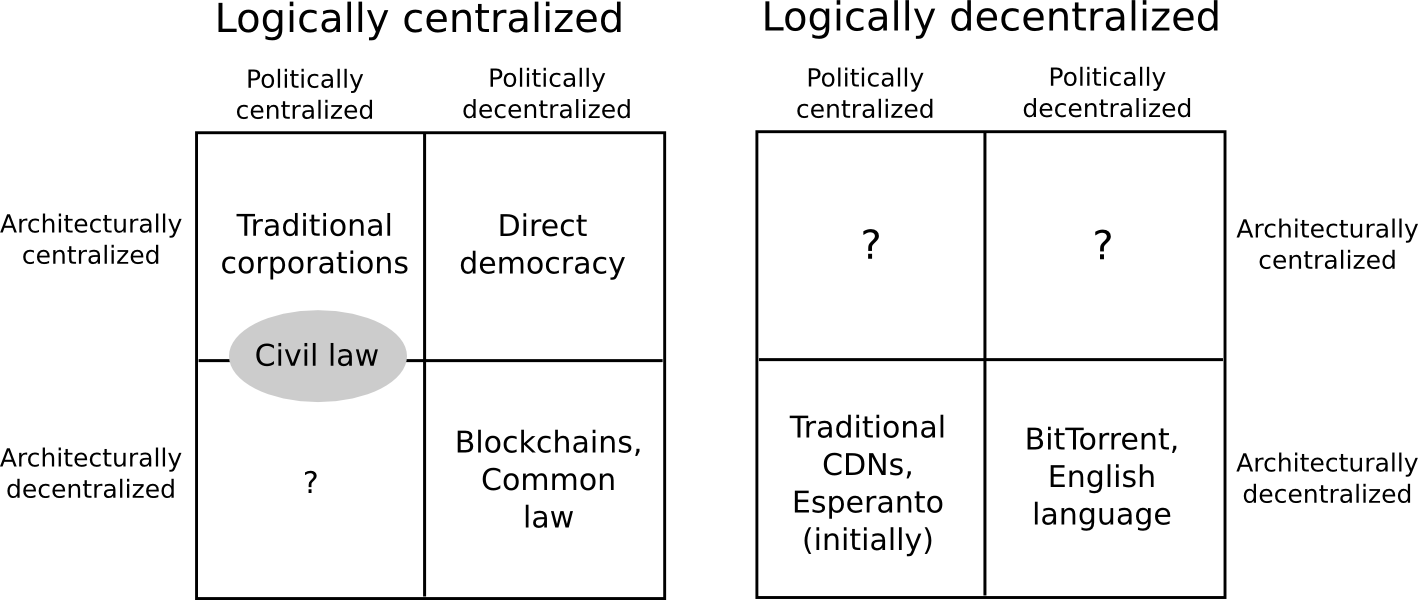
\includegraphics[width=1\textwidth]{immagini/meaning_decentralization.png}
\caption{Gli assi della decentralizzazione}
\label{fig:mesh1}

\end{figure}

Secondo l’autore, come illustrato nella figura 2.1, le blockchain sono architetturalmente e politicamente decentralizzate (nessuno esegue un controllo diretto su di esse e non c’è un punto centrale di guasto) ma logicamente centralizzate in quanto sono soggette a un preciso stato condiviso al momento dell'esecuzione del sistema che si comporta come un singolo computer\footfullcite{vitalButerinDecent}. Quest’ultimo aspetto, di nuovo, è fortemente legato ai protocolli di consenso che dipendono principalmente dalle varie tipologie di blockchain (un aspetto discusso nel paragrafo 2.4). La decentralizzazione riguarda maggiormente l’aspetto dei permessi dei partecipanti e governance sulla rete. La suddivisione descritta è valida per blockchain pubbliche (permissionless) sulle quali si concentra questa tesi, in cui tutti i partecipanti hanno pari diritti di agire e modificare il registro condiviso. Per quanto riguarda la tipologia delle blockchain con permessi (permissioned) la questione va riesaminata caso per caso a seconda dell’implementazione concreta. 

Uno tra tanti esempi di quest’ultima tipologia è Ripple\footfullcite{rippleMain}, blockchain per trasferimento di fondi che nel suo sistema di validazione si avvale di un certo numero di attori imposti a priori perché ritenuti fidati dall'azienda. Questa politica comporta dei vantaggi dal punto di vista della scalabilità e velocità di funzionamento a discapito della decentralizzazione dovuto alle forme di mediazione centralizzata. Attualmente, in questo specifico caso, con l’evoluzione della tecnologia blockchain questa strategia\footfullcite{rippleStrategy} viene rivista a favore di una maggiore decentralizzazione. Gli aspetti pro e contro l’adozione di sistemi più o meno decentralizzati sono discussi nel paragrafo (2.3.3).

Finalmente, distinte queste due nozioni è possibile arrivare alla seguente conclusione: il paradigma blockchain è distribuito (i partecipanti sono in possesso del registro replicato) mentre a livello inferiore, di implementazioni possono essere più o meno decentralizzate (o centralizzate) a seconda degli obiettivi e funzionalità che intendono raggiungere.

\subsection{Transazioni e concatenazione di blocchi}

Le blockchain utilizzano, letteralmente, una struttura pensata come una catena di blocchi. Ciascun blocco contiene al suo interno una lista di transazioni immutabili a loro volta contrassegnate da delle proprietà. Nelle attuali implementazioni le proprietà fondamentali sono:

\begin{itemize}
\item indirizzo mittente (input) 
\item indirizzo destinatario (output)
\item ammontare di valuta o token contenuto nella transazione
\item marcatura temporale (timestamp)
\end{itemize}


In una rete di consenso decentralizzato vengono man mano inseriti dei blocchi contenenti al loro interno un certo numero di transazioni. A livello universale, di rete, questa catena viene gestita dagli algoritmi di consenso come ad esempio: Proof of Work e Proof of Stake (descritti nel paragrafo 2.1.4) appendendo i blocchi giudicati validi dopo l'ultimo blocco valido della catena in modo da creare un registro di operazioni ordinato cronologicamente. Una volta stabilita la legittimità di un blocco e la sua appartenenza alla catena valida più lunga, l’intera struttura viene aggiornata propagando i nuovi elementi a tutti i partecipanti del sistema. Lo stato del registro a questo punto, non è più soggetto a modifiche, diventa permanente e immutabile. Successivamente, il procedimento riparte ricorsivamente, come descritto, ampliando la catena con le nuove operazioni.

Il primo blocco\footfullcite{genesisBitc} \smallskip \footfullcite{genesisEth} (hardcoded), originario di tutta la catena è chiamato \emph{genesi}. È un blocco speciale perché non è preceduto da altri blocchi, in esso vengono programmate le proprietà dei blocchi futuri. Le specifiche cambiano a seconda dell’implementazione. Generalmente, si tende a definire proprietà come la grandezza del blocco, la difficoltà di appendere nuovi blocchi e la ricompensa per la creazione (validazione) di nuovi blocchi nel sistema. 
Seguendo questo ragionamento, il seguente è un esempio valido di un blocco generico che eredita le sue proprietà dal blocco genesi.
Di seguito, insieme alle spiegazioni di alcuni concetti si forniscono pezzi di codice (code snippets) per illustrare la relativa struttura semplificata (il codice rispetta la sintassi Javascript ECMAScript 2015\footfullcite{jsDocs}). 
\\

\begin{lstlisting}[caption={Esempio di struttura di un blocco},language=JavaScript]
class block {
    constructor(timestamp, transactions, prevHash ='') {
        this.timestamp = timestamp;
        this.transactions = transactions;
        this.prevHash = prevHash;
        this.hash = this.calculateHash();
        this.nonce = 0;
    }
\end{lstlisting}

Ancora una volta, tra le proprietà importanti per il protocollo, si possono distinguere: la marcatura temporale che corrisponde alla data di creazione del blocco, la lista di transazioni incluse nel blocco, e la connessione tra i blocchi ovvero il "legame" calcolato tramite la funzione hash tra il blocco successivo e precedente.

Combinando insieme i blocchi si otterrà la seguente panoramica della struttura:

\begin{figure}[H]
\centering
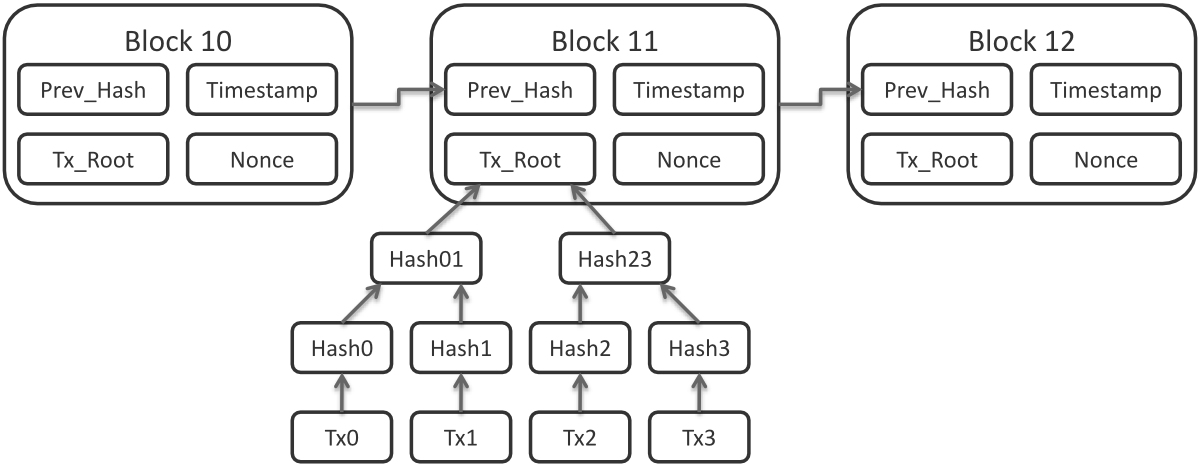
\includegraphics[width=1\textwidth]{immagini/bitcoinblocks.png}
\caption{Struttura semplificata di una catena di blocchi}
\label{fig:mesh2}

\end{figure}

Tenendo in mente che l'impostazione di un blocco può contenere un numero di proprietà variabile (a seconda dell'implementazione), è possibile generalizzare una struttura come quella illustrata nella figura 2.2. Nelle sezioni successive saranno analizzati gli elementi costituenti dei blocchi e le procedure che ne determinano il funzionamento.

\subsection{Funzioni di hash}

Ogni blocco è legato al blocco precedente tramite una funzione hash calcolata in base alle proprietà del blocco. Una funzione hash è una funzione matematica unidirezionale che accetta un input di lunghezza arbitraria e ne produce un output di lunghezza prefissata.

È una delle componenti base di una struttura formata da sequenze di blocchi che a sua volta è paragonabile alla struttura di una lista concatenata (linked list) tramite puntatori. In entrambi i casi la struttura permette di identificare in maniera univoca la relazione precedente e successivo che intercorre tra due blocchi. Dunque, data la definizione della funzione hash il suo risultato dipende dalle proprietà di ciascun blocco.

Senza entrare troppo in dettaglio, questo implica un insieme di proprietà "grande" sulle quali vengono calcolate le funzioni hash con la caratteristica che anche una minima variazione di ciascun componente del dominio della funzione molto probabilmente farà cambiare radicalmente il risultato calcolato.
Nel seguente esempio si calcola la funzione hash applicando l'algoritmo SHA256 (Secure Hashing Algorithm)\footfullcite{sha2Wiki}, utilizzata nelle blockchain (per esempio Bitcoin) per due input apparentemente simili: 
\\

\begin{lstlisting}
//Input 1: ciao Tizio
>> SHA256("ciao Tizio")
//Output 1: 
>> 875647588afa538ef3645bcdf413497af42461ea09e8f79df69b7a95c229d2a5
//Input 2: ciao tizio
>> SHA256("ciao tizio")
//Output 2: 
>> 961e89e74136c7094097f1a625b596f5df27cc6a71e0031bacf609e09feb2634
\end{lstlisting}

Si vede che anche la più piccola variazione in input produce (con probabilità estremamente alta) un output (righe 4,8) molto diverso.\footfullcite{hashExample}
Continuando con questo ragionamento, i blocchi sono formati da un insieme di proprietà che messe insieme produrranno una hash unica. Considerando il seguente esempio di calcolo della proprietà prevHash di un blocco:
\\
\begin{lstlisting}[caption={Esempio di calcolo della funzione hash in base alle proprietà del blocco},language=JavaScript]
>> SHA256(prevHash+timestamp+transactions+nonce)
\end{lstlisting}

È chiaro, a questo punto cosa si intende per quello che all'inizio di questa sezione veniva chiamato: "un'insieme di proprietà grande". Con più precisione, in qualsiasi blocco, il dominio della funzione hash è formato da (sempre in riferimento all'esempio della figura 2.2): marcatura temporale, il risultato delle continue applicazioni di hashing proprie di ciascuna transazione (tx root), il numero pseudocasuale (nonce) e il risultato della funzione hash del blocco precedente. In breve, vengono messe insieme tutte queste informazioni (paragonabile a una “polpetta” fatta da un composto di altri “elementi”) contenute nel blocco per produrre un unico hash. Questo, non è l'unico caso in cui l'utilizzo di questa funzione è fondamentale, l'hashing delle transazioni è stato menzionato per introdurre un livello di dettaglio ulteriore. Nella prossima sezione, a proposito delle continue applicazioni delle funzioni hash, verrà introdotta la struttura, Merkle Tree (albero di hash). 

Infine, disponendo della vista d'insieme dell'algoritmo di hashing, deriva la sicurezza dell'intero sistema. Supponendo uno o più attacchi con l'obbiettivo di alterare il contenuto dei blocchi. Il malintenzionato dovrà ricalcolare tutti gli hash dei blocchi successivi per validare l'intera catena e dovrà farlo prima che un nuovo blocco arrivi validato dal sistema di consenso. Di nuovo, in questo caso la priorità è della catena più lunga quindi l’eventuale attaccante sarà costretto a ricalcolare gli hash della nuova catena dall’inizio. Quello della sicurezza è un concetto che dipende dal sistema di consenso implementato e verrà discusso in seguito con maggior dettaglio.

\subsection{Merkle Trees}

Gli alberi di hash sono una struttura dati utilizzata nelle blockchain. È una delle componenti del blocco le cui proprietà fondamentali si sono ipotizzate negli esempi delle sezioni precedenti. In particolare, nella figura 2.2 è presente la radice (tx root) di un merkle tree. La radice è il risultato di applicazioni continue di operazioni hash a partire dal livello con cardinalità più alta (ipotizzando che la cardinalità della radice sia minore di quella dei suoi figli). Il motivo per cui viene usata questa struttura è da ricondurre all'efficienza degli alberi di hash, nel memorizzare, nel caso delle blockchain, le transazioni. 


\begin{figure}[H]
\centering
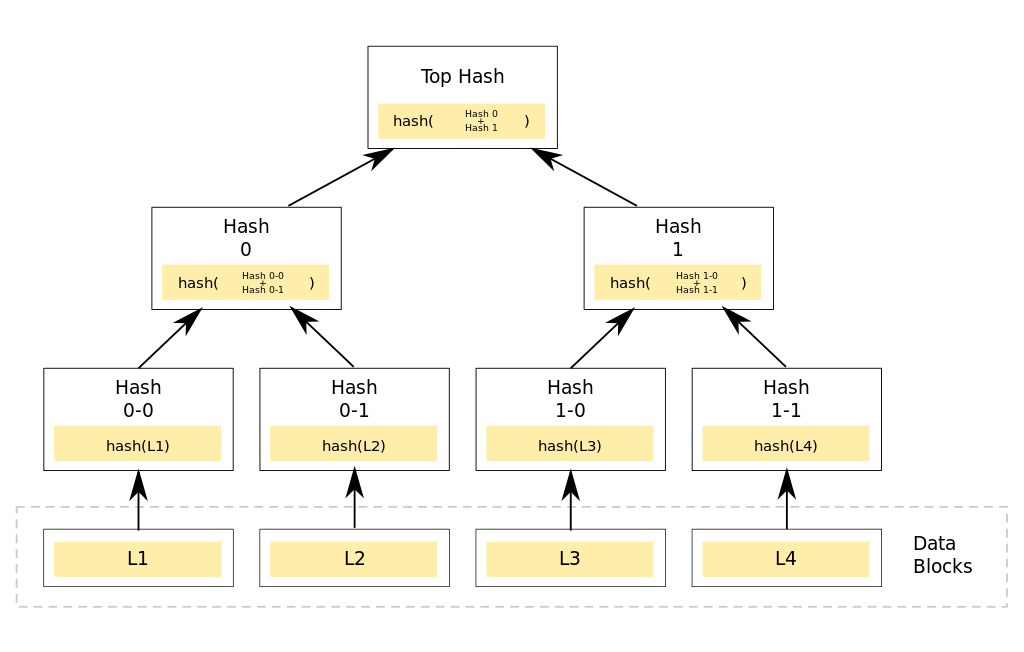
\includegraphics[width=1\textwidth]{immagini/hash_Trees.png}
\caption{Struttura di un merkle tree}
\label{fig:mesh3}

\end{figure}

La figura 2.3 rappresenta un albero di hash binario che può essere generalizzato per visualizzare il procedimento di hashing di un numero arbitrario di transazioni (limitate nella definizione del blocco). Nell'esempio a partire dal basso (o a livello di cardinalità più alto, nelle foglie) si trova contenuto l'insieme delle singole transazioni (L1-L4).

Il primo passo, consiste nell’eseguire l'algoritmo di hashing sulle singole transazioni. L'output di queste operazioni viene successivamente accoppiato con il risultato dell'elemento (nodo) adiacente e su di essi viene di nuovo eseguito l'algoritmo di hashing. Il procedimento è ripetuto ricorsivamente fino a giungere alla radice, risultato di continue applicazioni di hashing nell'insieme di nodi, i quali si trovano a sinistra e destra rispetto alla radice. Dunque, ogni nodo è l'hash dei suoi due figli\footfullcite{ethWhitepaper}. 

Una delle proprietà delle funzioni crittografiche di hash (come SHA-2) consiste, dal punto di vista computazionale di essere veloce da calcolare su qualunque tipo di dato. Inoltre, la peculiarità di questa struttura è che appendere nuove foglie, equivalenti a nuove transazioni che vengono man mano aggiunte all’albero, non comporta la ricomputazione dell’intera struttura ma solo del percorso che porta direttamente alla radice.

Il vantaggio dal punto di vista dell'efficienza dei merkle trees deriva proprio da questa impostazione della struttura gerarchica definita dagli elementi sottostanti. Si tratta dell'efficienza in termini di tempo e dello spazio necessario per memorizzare la struttura. La finalità di Merkle Tree deriva dalla frammentazione dei dati al suo interno e la loro composizione nella radice, sotto un unico identificatore hash. In questo modo per assicurare l'integrità del blocco sarà sufficiente per un nodo verificare la radice della struttura (tx root). Questo è possibile perché la propagazione con la messa insieme di funzioni hash avviene sequenzialmente dalle foglie alla radice.

A livello della blockchain questo apre diverse possibilità di verifica dell'integrità delle singole transazioni e la possibilità di ridurre lo spazio e il tempo necessario per sincronizzare la catena dei blocchi aggiornata all'ultima versione valida. Ad esempio, per un membro della rete che non intende effettuare operazioni su singole transazioni dei blocchi passati sarà sufficiente verificare solo gli hash contenuti nell'intestazione (header) dei blocchi. Se la sincronizzazione, il ricalcolo delle funzioni hash avviene con successo, questo implica l'appartenenza a una catena valida.

\section{Il sistema di consenso} %  Inizio sezione 2.1

Una volta definito il funzionamento concettuale di una rete blockchain. Sorge il dubbio come questo proliferare di operazioni, di calcolo delle funzioni hash, dell'addizione dei nuovi blocchi alla catena e più in generale l'insieme delle operazioni di gestione dell'intera struttura sia possibile in un ecosistema decentralizzato. 

Innanzitutto, le blockchain decentralizzate operano in maniera incentivizzata. La disintermediazione è garantita dagli algoritmi di consenso che stabiliscono le regole di funzionamento della rete. Nel caso delle blockchain pubbliche, si tratta di una rete dove tutti i partecipanti sono alla pari, possono proporre nuove transazioni e tutti insieme devono mettersi d'accordo su quali transazioni effettivamente aggiungere al registro comune. Si vede delineato qui un contesto in cui è presente un insieme di partecipanti ciascuno avente i propri interessi ma nonostante obiettivi spesso contrapposti l'intero sistema deve giungere a un consenso. Tipicamente, l'incentivizzazione consiste in una ricompensa, una quantità di valuta o token, spettante al nodo o ai nodi a cui viene dato il potere di appendere un blocco alla catena. L’approfondimento di questo aspetto economico è strettamente legato al tipo di algoritmo di consenso implementato, alcuni dei quali (ad esempio, Proof of Work e Proof of Stake), verranno discussi più avanti in questa sezione.

\subsection{Il problema dei generali bizantini}

Dal punto di vista teorico, la difficoltà di consenso può essere ricondotta al problema dei generali bizantini\footfullcite{byzantine-generals-problem}. In una delle possibili formulazioni del problema, si suppone che una città venga assediata da molti eserciti con a capo un generale. Per ottenere la vittoria tutti gli eserciti devono raggiungere un consenso e attaccare simultaneamente altrimenti se non attaccano in numero sufficiente verranno sconfitti. Il generale manda l’ordine, attraverso dei messaggeri ai comandanti degli eserciti che a loro volta possono mentire scegliendo arbitrariamente di passare ordini diversi e tradire il generale e gli altri comandanti.

Dunque, è una situazione che si porta bene a essere visualizzata all'interno delle blockchain (propriamente decentralizzate). In riferimento al problema sopra esposto si fa a meno del generale che manda degli ordini ai suoi sottoposti. Nella pratica, si tratta di una rete dove tutti i partecipanti possono proporre nuove transazioni e tutti insieme devono mettersi d'accordo su quali transazioni effettivamente aggiungere al registro comune in mancanza di un nodo generalmente definibile come detentore della verità (holder of truth). Il punto chiave è che tutti i componenti del sistema devono prendere la stessa decisione (e non necessariamente la decisione ritenuta “giusta”) su un piano di parità cioè senza l’esistenza di un’entità “fidata” che possa provarne l’autenticità. Tutto questo in un contesto di presenza di potenziali nodi "traditori" che minacciano l'integrità della rete. In riferimento a questi nodi viene sollevata la questione della fiducia che deriva dall'implementazione delle regole di consenso. La struttura delle blockchain (l’aggiunta di nuovi blocchi quindi la validazione delle transazioni) è controllata da queste regole le cui implementazioni implicano anche l'esistenza di un limite che se superato permette di approvare operazioni illecite e potenzialmente corrompere l'intera rete. Questo limite, a seconda dell’algoritmo utilizzato, riguarda la potenza computazionale necessaria per superare il controllo di validazione e il numero di nodi che decidono di mettersi d'accordo per approvare operazioni al di fuori dalle regole del sistema. Un esempio concreto, nella rete Bitcoin, la potenza computazionale necessaria per compromettere la rete è maggiore del 50\% totale della capacità computazionale dell’intera rete\footfullcite{btcAttacchi1}. Questa soglia, cresce man mano che i potenziali attaccanti vorrebbero modificare le transazioni contenute nei blocchi precedenti\footfullcite{btcAttacchi2}.

In questo modo, grazie al consenso distribuito, le blockchain riescono a rimediare al problema dei generali bizantini (BFT, Byzantine Fault Tolerance) in un ecosistema distribuito. Questo, come già accennato è garantito dagli algoritmi di consenso implementati nella rete, di cui i principali Proof of Work e Proof of Stake. Nell’insieme BFT contribuisce alla sicurezza della rete e previene il fenomeno della doppia spesa \footfullcite{btcSicurezza}.


\subsection{Proof of Work}

Proof of Work, cronologicamente, è il primo sistema di consenso usato nelle blockchain. Implementato per la prima volta da Bitcoin con lo scopo di raggiungere un consenso tra in nodi presenti sulla rete circa lo stato dell’intero sistema. La sua finalità consiste nella gestione e aggiornamento della catena dei blocchi con i relativi elementi in modo che i tutti i partecipanti siano “in linea” con la versione della catena valida cioè la sequenza dei blocchi più lunga. Il legame tra i blocchi una volta validato dall'algoritmo comporta la creazione di una struttura di contenuti immutabile contente tutta la storia delle operazioni intercorse fin dalla creazione del blocco genesi.
\begin{figure}[H]
\centering
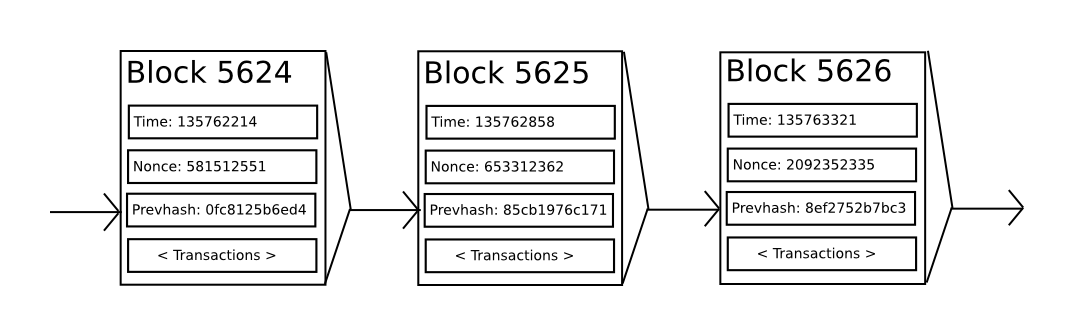
\includegraphics[width=1\textwidth]{immagini/mining_pow.png}
\caption{Mining: Proof of Work}
\label{fig:mesh4}
\end{figure}

Nella figura 2.4 è illustrato il processo di creazione di nuovi blocchi collegati mediante il riferimento all'indirizzo hash del blocco precedente. Da notare: il tempo di creazione del blocco strettamente crescente dovuto al funzionamento di Proof of Work che sequenzialmente, a intervalli regolari permette l'inserimento nella rete di un blocco valido. Messe insieme: la quantità di computazione richiesta e la creazione di blocchi a intervalli regolari permette di rimediare ai problemi di congestione della rete dovuti alla creazione di una quantità di transazioni troppo grande da essere processata in tempi ragionevoli (così come avviene negli attacchi di tipo DDOS).

Senza un punto centrale di calcolo, il procedimento di validazione è incentivato per permettere il funzionamento affidabile e costante in un sistema distribuito. Nel caso di Proof of Work, i membri della rete blockchain possono partecipare a una competizione con l’obbiettivo di appendere un blocco alla catena e ricevere in cambio una ricompensa. Si tratta di dimostrare di aver compiuto una quantità di calcoli computazionali per mezzo di cosiddetti “puzzle crittografici”. Queste dimostrazioni possono, ad esempio sfruttare la caratteristica della distribuzione uniforme delle funzioni crittografiche di hash per cui il calcolo di una funzione hash comporta la generazione di un risultato, il quale, come dimostrazione, dovrebbe appartenere a un insieme ristretto del dominio dei possibili risultati. Relativamente alla crescita e incremento della potenza computazionale dei calcolatori è consigliabile che questa dimostrazione sia controllata da una difficoltà variabile, anch’essa crescente in relazione all’aumento di hashrate (la frequenza di calcolo della funzione hash). Ad esempio, una dimostrazione Proof of Work, potrebbe richiedere che un numero arbitrario di cifre del risultato generato dalla funzione hash sia uguale a zero. Successivamente, l’incremento della difficoltà consiste nell’incremento di questo numero di cifre. Di conseguenza, l’aumento di hashrate è direttamente proporzionale alla probabilità di venire selezionati come creatori del nuovo blocco e quindi ricevere la ricompensa.

Per ribadire quanto è stato appena detto, si suppone che la dimostrazione richieda che le prime tre cifre della funzione hash calcolata siano pari a zero.
A questo scopo si riprende l'esempio del codice 2.3: Esempio di calcolo della funzione hash in base alle proprietà del blocco. 
\\
\begin{lstlisting}[caption={Esempio di calcolo della funzione hash in base alle proprietà del blocco},language=JavaScript]
function calculateHash(difficulty) {
    nonce = nonce + 1;
    return SHA256(prevHash+timestamp+transactions+nonce);
}
...
//Output per nonce = 10:
3747cd1b31b876bda0bf8540ad4eeb115239c2d69835a74cc5835d9d3b3f3b27
//Output per nonce = 11:
aac295677f4761d411bc4fdb2953ac3ce2a2b8202207928a8db1cdac45aa8885
...
//Output per nonce = 10390:
0000b280f48a4640ea18e2b6ee999fc60bfc85b690e990c0bdc4f9ae2b1e13c6

\end{lstlisting}

A ogni iterazione viene generato il risultato della riga 3 e successivamente confrontato con la difficoltà che in questo esempio supponiamo sia pari a 4. Concretamente, il numero di questi tentativi fatti in un secondo prende il nome di hashrate. Se il risultato non soddisfa la dimostrazione allora viene incrementata di uno la proprietà nonce, numero arbitrario che può essere usato una volta sola. Siccome, anche una minima variazione in input probabilmente farà cambiare radicalmente il risultato, ad un certo punto verrà generata un risultato che soddisfa i requisiti prestabiliti nella proprietà della difficoltà. Nella simulazione effettuata utilizzando una versione estesa di calculateHash l'output della riga 12 è stato trovato, dopo pochi secondi, al 10.390 tentativo. Per ottenere il risultato con cinque cifre iniziali uguali a zero ci è voluto quasi un minuto e 426.203 tentativi.

\begin{figure}[H]
\centering
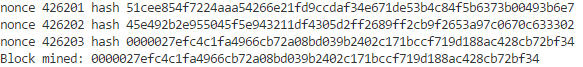
\includegraphics[width=1\textwidth]{immagini/miningOutput.png}
\caption{Mining: Risultato simulazione}
\label{fig:mesh5}
\end{figure}

In conseguenza, nelle applicazioni reali, succede che questa dimostrazione di calcoli computazionali porta con sé il consumo di una quantità enorme di energia elettrica. Evidentemente, può essere considerata come uno spreco con un impatto negativo su nei vari contesti generali come l’ambiente, la favorizzazione di utenti con infrastruttura più efficiente (ad esempio, mining pools) ecc.
Si ipotizza che, attualmente il consumo di energia annuo di Bitcoin sia di circa 2.55 GW paragonabile al consumo annuo dei paesi come l’Irlanda (circa 3.1 GW) e in questa forma è destinato a crescere\footfullcite{btcEnergy}.

\subsection{Proof of Stake}

Per contrastare le conseguenze negative derivanti dall’utilizzo di Proof of Work sono stati sviluppati oppure sono in produzione altri sistemi di consenso. Il perno della costruzione di questi sistemi riguarda proprio la fase di dimostrazione che contribuisce alla sicurezza e integrità della rete, così come descritta in Proof of Work. Tra i sistemi più promettenti è stato definito Proof of Stake, il quale riesce a risolvere il problema di consumo incrementale di energia dovuto alla quantità di calcoli computazionali.

Questo algoritmo si basa su un processo di elezione. All’interno della rete blockchain, gli utenti possono scegliere di entrare a far parte di un gruppo di utenti, aperto a tutti, chiamati validatori. Per poter partecipare a questo processo è sufficiente depositare una quantità di valuta o token che verrà conservata nella rete come deposito (stake). Analogamente a Proof of Work a ogni partecipante, nel caso di Proof of Stake chiamato validatore al posto di miner, viene concesso il potere di appendere un blocco alla blockchain ricevendo in cambio una ricompensa (di solito una parte delle commissioni incluse nell’insieme delle transazioni del blocco). Il nodo validatore può essere scelto seguendo un processo di selezione casuale e tenendo conto della quantità del deposito messo a disposizione. I vantaggi di questo approccio sono evidenti dal punto di vista dell’efficienza computazionale. Inoltre, con la crescita della rete e la quantità di criptovaluta circolante al suo interno diventa teoricamente impraticabile effettuare un attacco della maggioranza che tra le altre cose può essere ulteriormente contrastato introducendo una certa variabile di casualità al processo di selezione del validatore. La scelta di particolari soluzioni dipende dalle diverse implementazioni dell'algoritmo, relativamente a Proof of Stake è opportuno menzionare che il deposito di validatori disonesti cioè coloro che cercano di approvare transazioni fraudolente non sarà restituito e in tal caso perderebbero dei soldi. Lo stesso deposito sarà mantenuto dalla rete per un certo periodo di tempo necessario per provare che non siano state accettate transazioni fraudolente da parte del validatore.

% Fine sezione 2.2

\section{Funzionamento dell'ecosistema blockchain} % Inizio sezione 2.3

Lorem ute irure dolor in reprehenderit in voluptate velit esse cillum dolore eu fugiat nulla pariatur. Excepteur sint occaecat cupidatat non proident, sunt in culpa qui officia deserunt mollit anim id est laborum.

\subsection{Transazioni e prevenzione della doppia spesa}


Digital signatures, double spend

\subsection{Teoria dei giochi e governabilità}

hardforks

\subsection{Trilemma scalability}

\blindtext

\section{Tipologie di un sistema distribuito} %  Inizio sezione 2.2

Unpermissioned ledgers, Permissioned ledgers, A shared ledger

\subsection{Unpermissioned Ledgers}

\subsection{Permissioned Ledgers}

\blindtext

\section{Blockchain negli archivi digitali} %  Inizio sezione 2.2

% direi che non è necessario
%\section{Esempi di applicazione}

%\subsection{Case study 1: Santander money transfer}

%\subsection{Case study 2: Blockchain università di Pisa}

%\subsection{Case study 3: ?}
%\footfullcite{Haber91howto}
%\footfullcite{Kurose:2012:CNT:2584507}

\chapter{Ethereum: Sviluppo di applicazioni decentralizzate}

Seguendo la divisione a tre strati: di concetti, implementazioni e istanze definita fin dall'inizio del lavoro, in questo capitolo verrà affrontato l'aspetto dell'implementazione nel caso concreto della piattaforma Ethereum. I concetti spiegati fino a questo punto costituiscono un base decisionale, un punto di partenza per scegliere le implementazioni che meglio si adottano alle proprie necessità. I concetti presentati finora possono essere visti come una sorta di contenitore aperto da cui è possibile “pescare” le componenti concettuali da implementare a seconda delle funzionalità dell’applicazione reale. 

Importante sottolineare che lo stato dell'arte delle blockchain limita l’utilità di descrivere in dettaglio le implementazioni concrete. Questa affermazione deriva dal contesto attuale, le blockchain nonostante non siano più definibili come una tecnologia fra le più recenti in confronto alle tempistiche nel settore informatico, generalmente non hanno raggiunto una stabilità sufficiente. Usando la terminologia presente nelle analisi e predizioni annuali condotte dalla Gartner\footfullcite{gart} la blockchain si trova attualmente sulla via di uscita dal cosiddetto "hype cycle"\footfullcite{gart2016} \smallskip \footfullcite{gart2018}. Una metodologia usata per rappresentare la maturità, l'adozione e l'applicazione di nuove tecnologie.

\begin{figure}[H]
\centering
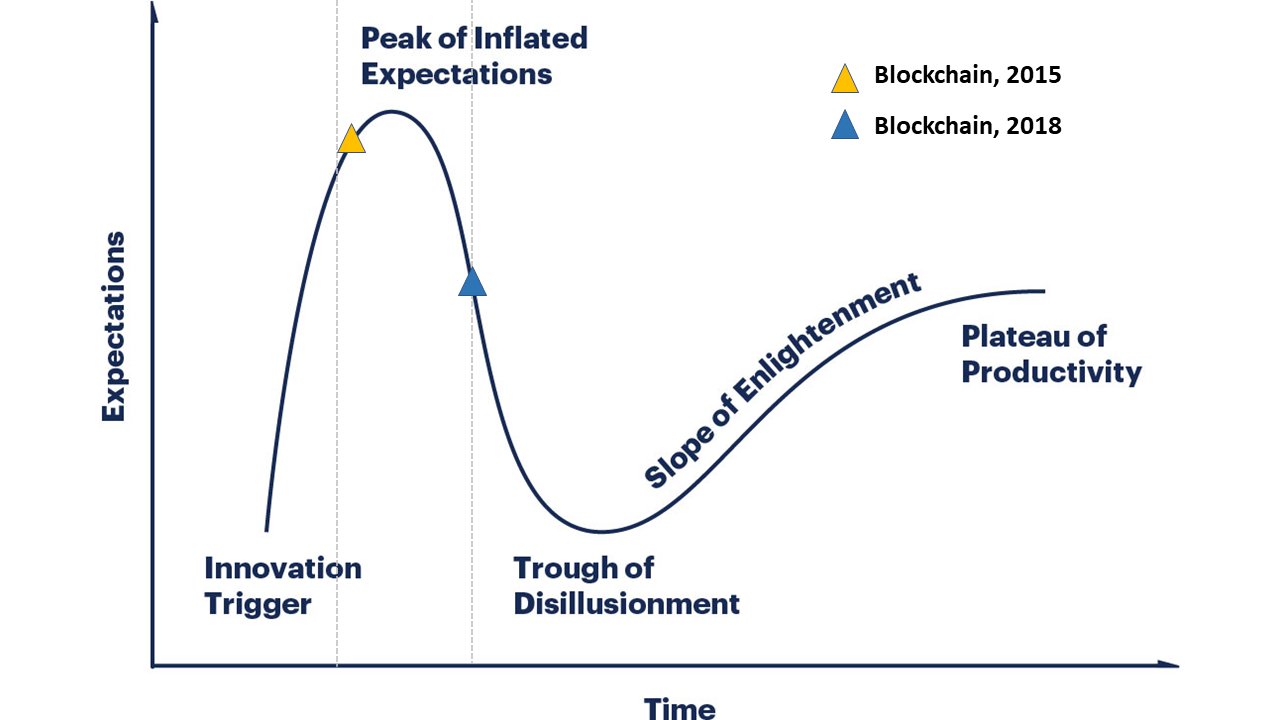
\includegraphics[width=1\textwidth]{immagini/blockchainHype.png}
\caption{Hype}
\label{fig:mesh7}
\end{figure}

La situazione può essere vista come un contesto variabile, di continuo sviluppo con l’emergere di nuove implementazioni, piattaforme e applicazioni. Una ricerca spesso finalizzata al miglioramento e adozione delle nuove tecniche per contrastare le limitazioni attuali del sistema ma pur sempre una situazione, qual è quella presente, in continuo mutamento caratterizzata dall'instabilità e in alcuni casi, cambiamenti radicali. Tuttavia, questo non pregiudica l’utilità delle cose dette finora in quanto si tratta di concetti fondamentali che, nel caso peggiore, possono servire anche per comprendere le scelte e gli sviluppi futuri. 

La scelta di Ethereum come sistema da presentare, collegato alla successiva costruzione di un’applicazione nel capitolo successivo è stata fatta seguendo tra le altre, queste motivazioni: di stabilità, sviluppo e innovazione. Viene perseguita l'idea legata alla correlazione tra il successo e la popolarità di un sistema misurata tenendo conto del numero di partecipanti e sviluppatori coinvolti, gli strumenti di sviluppo messi a disposizione e il loro grado di maturità, la frequenza di aggiornamenti e l’interesse della comunità ed enti pubblici e privati con i relativi rischi connessi. Un insieme di fattori che le nuove implementazioni dovranno cercare di raggiungere per attrarre gli utenti e gli sviluppatori ai loro sistemi. Al momento dello scrivere la piattaforma Ethereum è il sistema più sviluppato sotto l’aspetto di sviluppo delle applicazioni decentralizzate.

\section{Implementazione Ethereum}

Ethereum è una di piattaforma di sviluppo delle applicazioni decentralizzate basata sulla tecnologia blockchain pubblica e open-source.

La novità principale è data dalla possibilità di programmazione in maniera Turing Completa. Si tratta dunque, di una blockchain programmabile con un linguaggio chiamato Solidity attraverso cui è possibile esprimere qualsiasi algoritmo esprimibile con altri linguaggi di programmazione universali. Questi programmi scritti e compilati all’interno della blockchain prendono il nome di “Smart Contracts” e si comportano come dei contratti veri e propri. In rapporto ai loro corrispettivi tradizionali i termini contrattuali non sono definiti usando un linguaggio legale ma direttamente il codice dei programmi (chiamati appunto contratti). Gli smart contracts, permettono quindi l’impementazione della logica delle transazioni e inoltre permettono la disintermediazione tra le parti interessate grazie ai concetti che guidano le blockchain. 

Riassumendo, la visione del progetto Ethereum è quella di creare un computer decentralizzato permanente e autosufficiente in grado di resistere ai tentativi di censura. Dal punto di vista della programmazione, nella figura 3.2 è rappresentato il flusso relativo all’architettura di un’applicazione blockchain.

\begin{figure}[H]
\centering
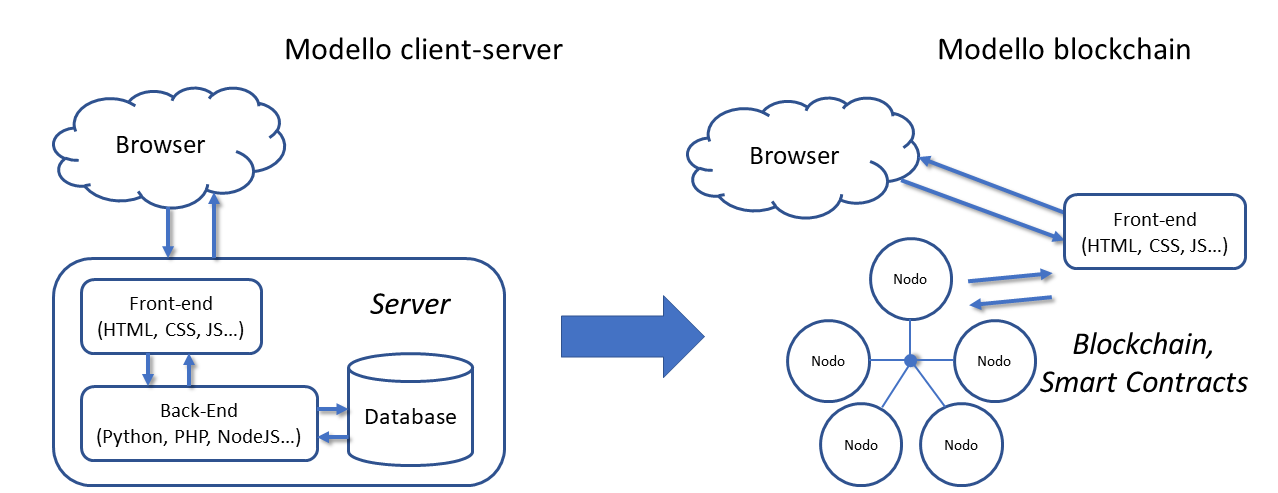
\includegraphics[width=1\textwidth]{immagini/architetturav1.png}
\caption{Architettura}
\label{fig:mesh8}
\end{figure}

In relazione al classico modello client-server, nel modello decentralizzato lo strato back-end è direttamente implementato nella blockchain attraverso gli smart contract situati direttamente sulla blockchain che a sua volta corrisponde a una base di dati con storia completa e distribuita su tutti i nodi. L’esecuzione della logica dei contratti avviene grazie alla macchina virtuale Ethereum (EVM) eseguita da ciascun nodo della rete.


In questo capitolo verranno ripresi i concetti presentati e le loro implementazioni concrete con le relative modifiche ed espansioni. Nella vista di insieme si parlerà di:

\begin{itemize}
\item Espansione del concetto di transazione
\item Struttura dati Patricia trees come espansione di Merkle trees
\item Funzioni hash Keccak
\item Sistema di consenso con il passaggio da Proof of Work in Ethereum Metropolis  a Proof of Stake nella versione Constantinople
\end{itemize}

Caratteristiche: 
- Permessi: è una blockchain pubblica, decentralizzata\\
- Hash: funzione di hash keccak256\\
- Struttura dati: Merkle Trees - patricia trees\\
- Sistema di consenso PoW\\
- Smart contracts\\
-- DA FARE\\

\subsection{Transazioni}

\subsection{Patricia Trees}

\begin{figure}[H]
\centering
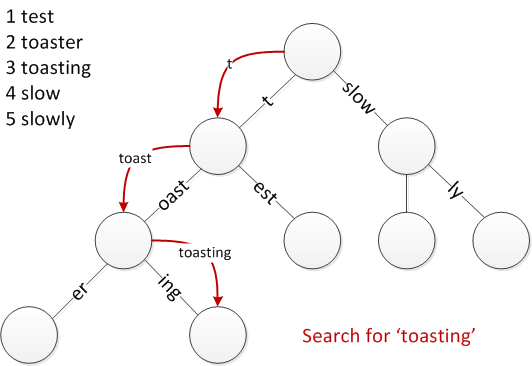
\includegraphics[width=1\textwidth]{immagini/patricia_trie.png}
\caption{Struttura di patricia trie}
\label{fig:mesh6}
\end{figure}

\subsection{Ethereum Metropolis e Constantinople}

Qui scrivo del consenso e della transizione da PoW a PoS
Magari anche forks?

\section{Smart Contracts}

\subsection{Solidity}

\subsection{Ethereum Virtual Machine}

\subsection{Gas}

\section{Data storage}
\chapter{Progetto di Archivi Digitali}
\label{ch:archivi}

Questo capitolo contiene la documentazione del progetto realizzato utilizzando le tecnologie descritte nei capitoli precedenti. Si tratta di un’applicazione decentralizzata costruita attraverso la blockchain pubblica Ethereum e il protocollo IPFS. Lo scopo principale di questo progetto è la descrizione della metodologia di sviluppo in un ecosistema distribuito. Se per molti programmatori imparare un nuovo linguaggio di programmazione o framework può essere una situazione frequente, lo sviluppo in un paradigma differente richiede una descrizione più approfondita della metodologia e delle pratiche migliori da adottare durante la fase di preparazione e di sviluppo.

\section{Definizione di obiettivi e requisiti dell’applicazione}

L’obiettivo consiste nello sviluppo di un'applicazione per la registrazione di opere d’arte definibili come \emph{minori} che, potranno essere memorizzate in maniera trasparente, permanente e immutabile in una blockchain pubblica.

In dettaglio l’applicazione deve soddisfare i seguenti requisiti e funzionalità:

\begin{itemize}
\item Inserimento di oggetti nell’archivio, descritti attraverso l’utilizzo di sistemi di metadati opportuni.
\item Memorizzazione e visualizzazione degli oggetti inseriti.
\item Possibilità di modificare l’oggetto inserito da parte del suo autore mantenendo la storia completa delle modifiche effettuate.
\end{itemize}

Gli utenti previsti per l'applicazione sono di due tipi:
\begin{itemize}
\item Qualsiasi utente dotato di un indirizzo sulla rete, quindi in grado di interagire con l'applicazione, può, senza restrizioni, visualizzare tutti gli oggetti inseriti nell'archivio. Inoltre finché l'utente dispone di fondi sufficienti potrà inserire nuovi oggetti e modificare la loro descrizione.
\item Utenti dotati di permessi di verifica e approvazione dei dati inseriti nell'archivio attraverso un sistema di votazione.
\end{itemize}

Tenendo in mente questi requisiti e le considerazioni fatte nel capitolo \ref{sectionDigitalArchives}: "Blockchain negli archivi digitali" è possibile procedere con l'implementazione basata sulla blockchain Ethereum.

\subsection{Sistemi di metadati}

Prima di proseguire con la fase dello sviluppo dell'applicazione, una considerazione importante riguarda la descrizione delle risorse attraverso sistemi di metadati. Secondo una descrizione generica: “i metadati sono informazioni strutturate relative ai dati, interpretabili da parte di un computer”\footfullcite{metadatiCNR}. Inserire un oggetto dentro un archivio digitale che gestisce opere d’arte minori implica l'implementazione di un sistema di regole adatto a esprimere le diverse tipologie delle risorse in questione. Ad esempio, le risorse da rappresentare possono essere dei manoscritti, delle fotografie, dei disegni, degli oggetti di oreficeria e così via.

Esistono molti standard più o meno formali per la descrizione di particolari categorie di materiale, per questo progetto si è scelto di implementare tre modalità di rappresentazione delle risorse, le prime due appartengono allo schema di metadati Dublin Core\footfullcite{dublinCore}, mentre la terza è un esempio del modello ontologico CIDOC Conceptual Reference Model (CRM)\footfullcite{cidocCRM}.

La scelta dei metadati è stata fatta tenendo conto di diversi fattori, innanzitutto si è cercato di scegliere gli schemi in grado di rappresentare il vasto insieme di tipologie a cui possono appartenere gli oggetti dell'archivio. Inoltre, nello scenario d'uso della salvaguardia dei beni artistici, potrebbe essere importante adottare un sistema utile alle forze dell'ordine (vedi il paragrafo successivo). Infine un’altra considerazione può essere fatta relativamente alla ricerca di un compromesso tra la complessità della descrizione, la facilità di utilizzo per un utente non esperto in materia e il grado di precisione del sistema utilizzato. Per questo l’utente può scegliere tra tre modalità di inserimento, dal più semplice al più complesso. Dublin Core fornisce uno schema di meta informazioni ideato per assegnare etichette ragionevolmente interessanti per qualunque materiale digitale. È uno schema flessibile, semplice ed estendibile che si presta bene alla costruzione di form adatte per la maggior parte dei casi di utilizzo previsti.

In figura \ref{fig:progettoInserimento} è rappresentata una parte della finestra contenente il modulo di inserimento, implementato nel progetto, con le scelte relative ai sistemi di descrizione da utilizzare.

\begin{figure}[H]
\centering
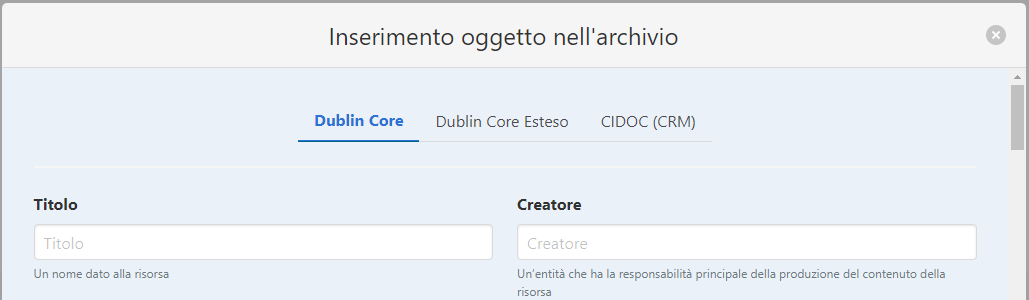
\includegraphics[width=1\textwidth]{immagini/inserimentoArchivio.PNG}
\caption{Progetto: Modulo inserimento nell'archivio}
\label{fig:progettoInserimento}
\end{figure}

La prima opzione, "Dublin Core", fornisce quindici etichette base per la descrizione delle risorse. La seconda opzione, "Dublin Core Esteso", permette una descrizione più approfondita della risorsa attraverso l'uso di qualificatori (o sottoclassi) che permettono un raffinamento dello schema con l'aggiunta di significati più precisi sui termini base. Infine la terza opzione, "CIDOC", è rivolta agli \emph{esperti} in quanto fornisce un modello ontologico formale incentrato sulla rappresentazione semantica delle risorse.

Un ultima considerazione pratica riguarda le linee guida per la descrizione di beni culturali, fornite dal nucleo carabinieri per la tutela del patrimonio culturale in figura \ref{fig:carabinieriTPC}.

\begin{figure}[H]
\centering
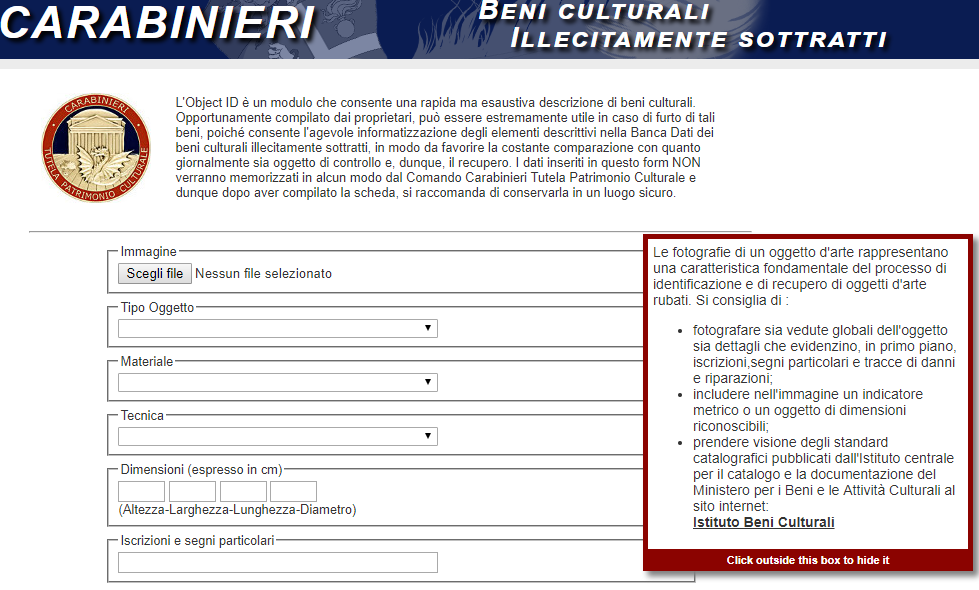
\includegraphics[width=1\textwidth]{immagini/carabinieriTPC2.png}
\caption{Beni culturali illecitamente sottratti: Modulo descrittivo}
\label{fig:carabinieriTPC}
\end{figure}

Il modulo Object ID\footfullcite{tpcCarabinieri}, adottato dalle forze dell'ordine, consente la descrizione di beni culturali ed è utile per le operazioni di recupero in caso di furto di tali beni. Quando la tecnologia sarà sufficientemente matura e testata, l'approvazione degli oggetti inseriti tramite un'applicazione basata sulla blockchain, potrebbe essere fatta dai membri autorizzati del Comando Carabinieri. Chiaramente il fatto di poter contare su una base di dati immutabile, permanente e dotata di storia completa fornirebbe dei vantaggi rilevanti rispetto ai sistemi attualmente in uso.

Con questo progetto si vuole dimostrare che è possibile adottare qualunque schema di descrizione in maniera relativamente semplice e quindi fornire una prova attendibile del possesso di tali beni. Mentre queste considerazioni sono state fatte tenendo in mente l'obiettivo consistente nella dimostrazione della metodologia, nel caso di un’applicazione pronta ad essere adottata al pubblico, questa parte assumerebbe un ruolo di primo piano per l'intero processo di sviluppo.

\section{Preparazione dell'ambiente di sviluppo}

Lo sviluppo del progetto sulla blockchain Ethereum è accompagnato dalla presenza di numerosi strumenti, in questa sezione sarà fornita la lista dei principali strumenti e delle dipendenze utilizzate durante la programmazione.

\begin{itemize}
\item NPM (Node Package Manager) per la gestione e l'installazione dei moduli/librerie Javascript. NPM richiede la presenza di Node.js\footnote{In questo progetto si è utilizzato Node.js nella versione 10.8.0 e NPM versione 6.2.0}.

\item Truffle framework (versione 4.1.14)\footfullcite{truffleFramework} un ambiente di sviluppo composto da un insieme di strumenti che facilitano la creazione delle applicazioni decentralizzate (di seguito dApps) sulla piattaforma Ethereum. Truffle gestisce il ciclo di migrazione (sulla blockchain) degli smart contracts, la loro integrazione ed esecuzione con la possibilità di eseguire test automatizzati.

Il framework include Ganache\footfullcite{ganache} (versione 1.2.2), una blockchain personale, utile per lo sviluppo locale delle dApps. Ganache è un emulatore di nodi Ethereum con un'interfaccia grafica intuitiva (in figura {\ref{fig:ganache}}), mette a disposizione un certo numero di account precaricati con Ether. Si tratta di una blockchain con un funzionamento semplificato che permette di analizzare lo stato della blockchain in qualunque momento dell'esecuzione.

\begin{figure}[H]
\centering
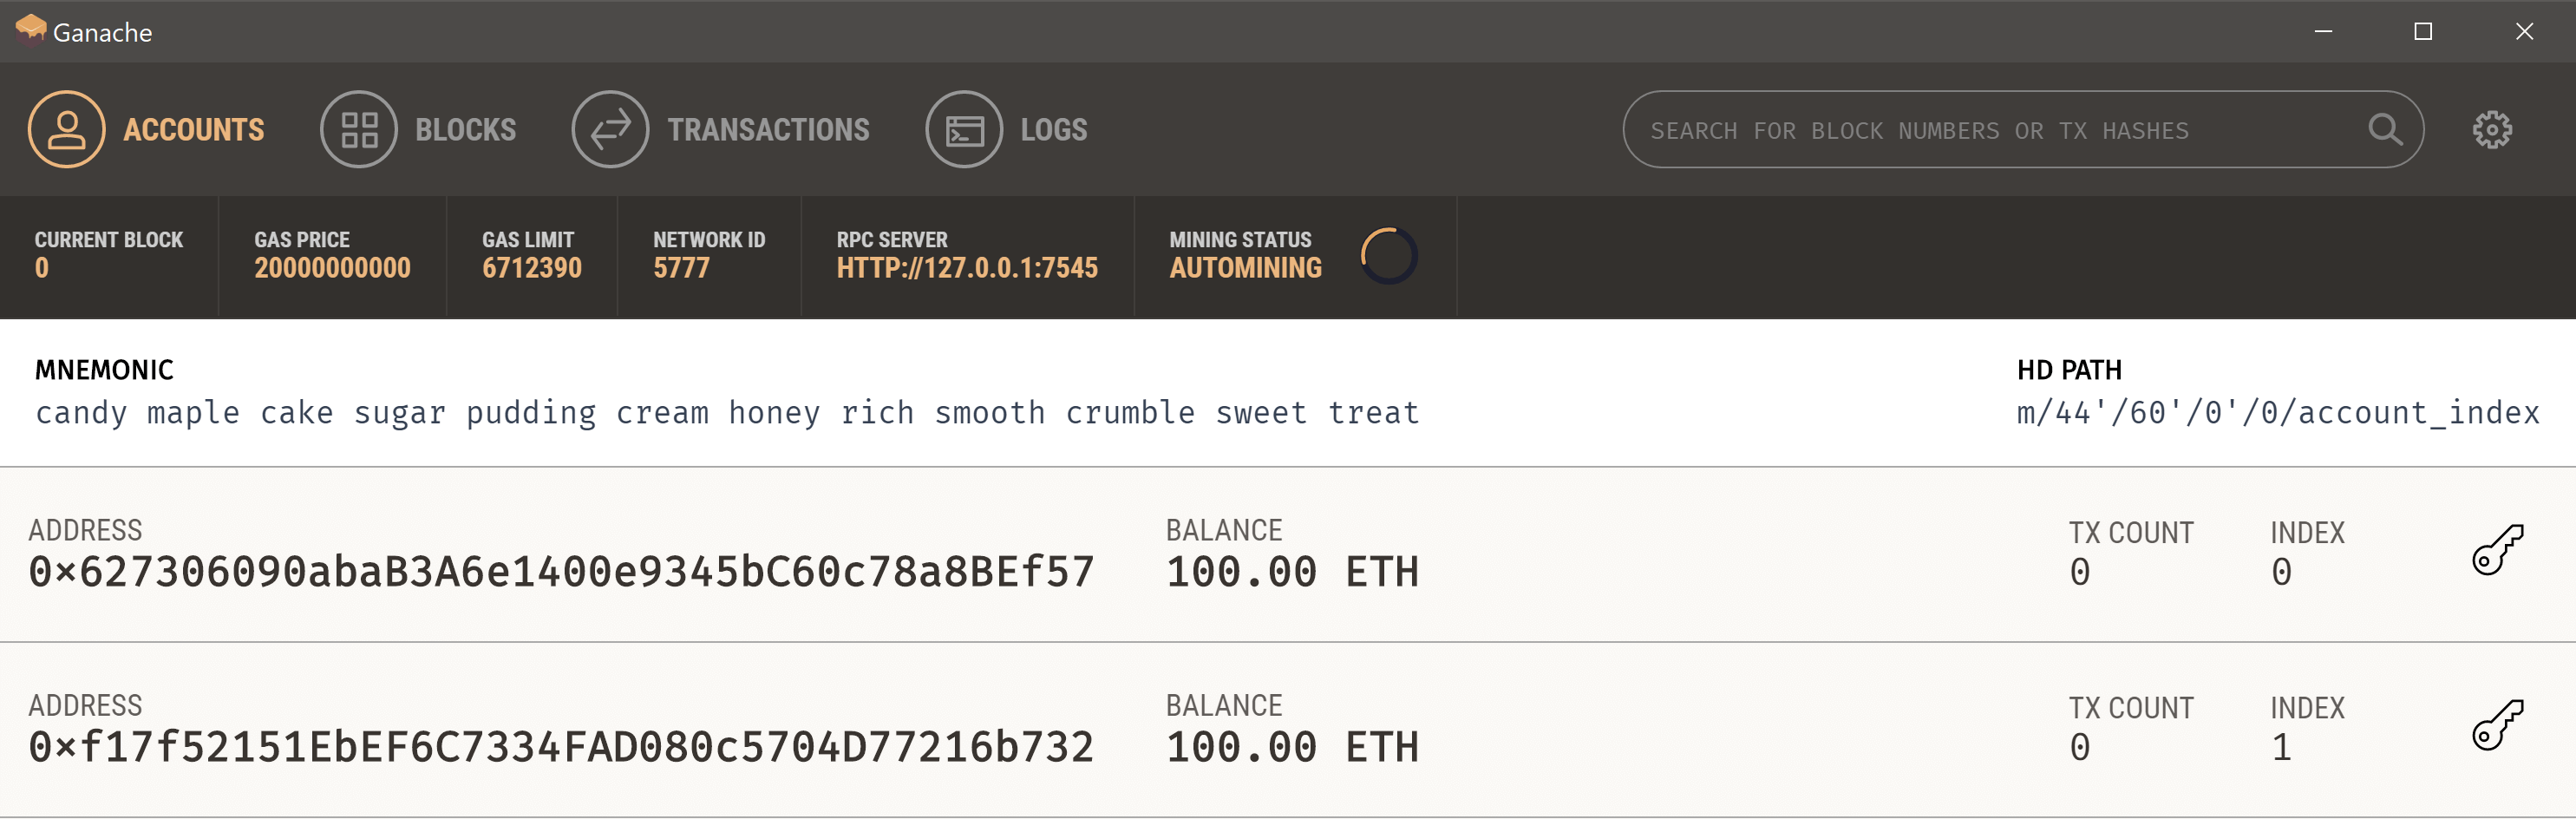
\includegraphics[width=1\textwidth]{immagini/ganache-window.png}
\caption{Ganache: Blockchain locale}
\label{fig:ganache}
\end{figure}

Truffle fornisce anche il codice \emph{boilerplate} raggruppato in diversi pacchetti chiamati "boxes", utili per uno sviluppo accelerato\footnote{Come base di questo progetto si è scelto il pacchetto chiamato pet-shop disponibile su https://truffleframework.com/boxes/pet-shop}.

\item Geth\footfullcite{geth} è l'implementazione ufficiale di un nodo completo Ethereum che permette la sincronizzazione e la partecipazione alla blockchain Ethereum.

\item Mocha e Chai sono usati per la creazione e l'esecuzione di test automatizzati. Mocha\footfullcite{mocha} è un test framework per Javascript basato su Node.js, mentre Chai\footfullcite{chai} è una libreria di asserzioni che può essere implementata sul framework. Insieme permettono l'implementazione di test automatizzati complessivi secondo un approccio TDD (Test Driven Development) e BDD (Behaviour Driven Development).

\item Metamask\footfullcite{metamask} è un’estensione, disponibile per i maggiori browser (Firefox, Chrome,Brave, ecc.). Necessario per utilizzare le dApps, fornisce un portafoglio (\emph{wallet}) che consente di identificare l'utente (attraverso la chiave pubblica) e di gestire le transazioni con la chiave privata.

\item Web3.js\footfullcite{web3} (versione 0.20) è una collezione di librerie che, attraverso un API, permette l'interazione con il codice dei contratti situati sulla blockchain. In particolare, permette di sviluppare la parte client dell'applicazione con le chiamate di lettura e di scrittura ai contratti.

\end{itemize}

Questi sono gli elementi più importanti, al momento più usati per interagire con le dApps e per sviluppare le proprie applicazioni. Altri elementi scelti per lo sviluppo di questa specifica applicazione, nella maggior parte opzionali, verranno introdotti in seguito.

\section{Sviluppo dell'applicazione}

Lo sviluppo di questo progetto può essere suddiviso in due fasi distinte:

\begin{itemize}

\item La prima fase si pone come obiettivo la creazione di un \emph{Minimal Viable Product} (MVP) cioè un prototipo che implementata le funzionalità base. Consiste principalmente nello sviluppo dei contratti, l'esecuzione di test e costruzione di un'interfaccia di prova (GUI) che permette l'interazione con i contratti in un contesto di sviluppo locale.

\item Nella seconda fase si estende l'applicazione in modo da implementare nuove funzionalità e costruire la versione finale. Questa fase consiste principalmente nell'integrazione con il servizio di storage IPFS, lo sviluppo della parte front-end finale e il trasferimento dei contratti su una blockchain Ethereum di sviluppo (\emph{testnet}).

\end{itemize}

\subsection{Scrittura dei Contratti}

Gli smart contracts scritti in Solidity costituiscono la parte back-end e contengono la logica dell'applicazione. Nel contratto principale, \emph{Archives.sol}, tra le prime operazioni si definisce la struttura degli oggetti da inserire sulla blockchain.
\\
\begin{lstlisting}[caption={Struttura degli oggetti},language=JavaScript]
struct Artwork {
    uint id; //identificatore univoco
    address author; //indirizzo dell'autore
    string name; //nome o titolo dell'oggetto
    string descriptionHash; //descrizione completa dell'oggetto
    string mainPreviewHash; //immagine rappresentativa dell'oggetto
    bool validation; //stato dell'approvazione (true o false)
    uint votesNum; //numero delle approvazioni (o voti)
}
\end{lstlisting}

Le caratteristiche degli oggetti sono definite tramite una variabile "Artwork" di tipo \emph{struct} cioè un tipo complesso definito dall'utente contenente al suo interno un insieme di proprietà che definiscono l'oggetto. Il passo successivo consiste nella costruzione di una sequenza di oggetti da memorizzare sulla blockchain. In Solidity è possibile costruire una sequenza composta da coppie chiave-valore (come in un array associativo) usando il tipo \emph{mapping}.
\\
\begin{lstlisting}[caption={Associazione chiave-valore},language=JavaScript]
mapping (uint => Artwork) public artworks;
uint artworkCounter; //contatore degli oggetti inseriti 
\end{lstlisting}

In questo modo il mapping crea una specie\footfullcite{solidityMapping} di tabella hash (inizialmente vuota\footnote{In realtà è impossibile determinare a priori la dimensione del mapping o eseguire direttamente delle iterazioni sugli elementi. Questo perché tutte le chiavi restituiranno un valore di default di tipo Artwork.}) composta da un indice univoco (uint) che si riferisce a un oggetto di tipo Artwork. Ogni volta che verrà eseguito un assegnamento di chiave-valore, il risultato sarà memorizzato sulla blockchain. Le tabelle hash sono una struttura dinamica e pertanto è necessario tenere una variabile di stato contatore in modo da tenere traccia degli oggetti effettivamente inseriti.

A questo punto analizzando il codice del contratto Archives.sol\footnote{https://github.com/lukasd2/Digital-Archives-dApp/blob/master/contracts/Archives.sol} sono state implementate le funzionalità descritte nella fase di definizione dei requisiti del progetto.
\\
\begin{lstlisting}[caption={Funzioni principali del contratto Archives.sol},language=JavaScript]
function publishArtwork(string _name, string _descriptionHash, 
                        string _dataHash) public {...}
function approveArtwork(uint _id) public onlyIfWhitelisted(
                        msg.sender) checkValidation(_id) {...}
function modifyArtworkDescription(uint _id, 
                        string _newDescriptionHash) public {...}
\end{lstlisting}

\begin{itemize}
\item La funzione "publishArtwork" gestisce l'inserimento di un nuovo oggetto nell'archivio.
\item La funzione "approveArtwork" gestisce l'approvazione degli oggetti inserti. Permette agli utenti autorizzati di votare per un dato oggetto e di controllare se il numero di voti registrati è sufficiente alla sua approvazione.
\item La funzione "modifyArtworkDescription" permette all'utente che inserisce l'oggetto di modificare la sua descrizione.
\end{itemize}

Successivamente al contratto Archives.sol sono stati aggiunti altri contratti che espandono le funzionalità e i controlli richiesti dall'applicazione. Per la costruzione della struttura dei contratti si è sfruttato il meccanismo dell'ereditarietà di Solidity, con la gerarchia rappresentata in figura \ref{fig:contractStructure}. Archives.sol si trova al livello più alto della catena e dunque può usufruire di tutte le funzioni definite nei contratti situati a livello più basso. In particolare i contratti Whitelist.sol, RBAC.sol e Roles.sol sono usati rispettivamente per aggiungere indirizzi alla lista di utenti dotati di permessi di verifica e per gestire i permessi degli utenti che acquistano lo status di "artwork checker" con i rispettivi controlli.
Il contratto Ownable.sol implementa il meccanismo di autorizzazione dell'autore del contratto, cioè all'indirizzo che pubblica il contratto sulla rete. Nella versione attuale al "proprietario" vengono dati i permessi di aggiungere nuovi utenti alla whitelist. 

\begin{figure}[H]
\centering
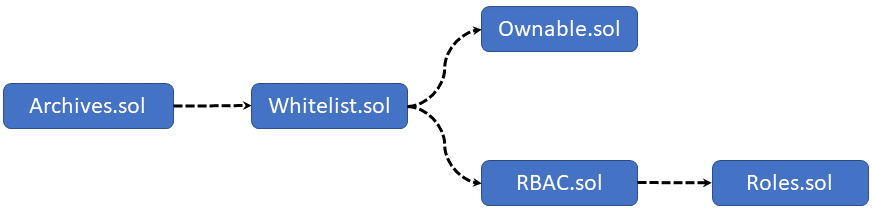
\includegraphics[width=1\textwidth]{immagini/contractStructure.png}
\caption{Progetto: Struttura dei contratti}
\label{fig:contractStructure}
\end{figure}

Questi contratti (Whitelist.sol, Ownable.sol, RBAC.sol e Roles.sol) sono stati presi dalla libreria OpenZeppelin\footfullcite{openZeppelin} contenente implementazioni delle funzionalità ricorrenti nelle dApps. Sono considerati sicuri perché ampiamente testati e aggiornati dalla comunità, questi contratti sono stati opportunamente modificati e integrati in questo progetto{\footnote{Codice di tutti i contratti implementati, https://github.com/lukasd2/Digital-Archives-dApp/tree/master/contracts}}.

\subsection{Test dei Contratti}

Una volta implementata la logica dell'applicazione è particolarmente importante assicurarsi che i contratti siano sicuri e privi di errori eseguendo dei test automatici. Gli smart contracts una volta pubblicati su Ethereum diventano immutabili, ai contratti verrà assegnato un certo indirizzo sulla blockchain e non sarà più possibile effettuare delle modifiche al loro codice a meno di caricarne altri sotto nuovi indirizzi.

Un altro aspetto importante riguarda i costi legati alla loro pubblicazione (\emph{deploy}), le nuove versioni dell'applicazione possono essere pubblicate sotto nuovi indirizzi e ogni volta sarà necessario pagare, ex novo, il prezzo (Gas) calcolato per la loro pubblicazione. Un discorso analogo può essere fatto per i costi legati alle singole transazioni del contratto, l'obiettivo ideale è quello di creare una versione dell'applicazione ottimizzata e affidabile per i casi d'uso previsti dal programma e allo stesso tempo testata per prevenire comportamenti indesiderati.

In questa applicazione i programmi di testing sono stati divisi in tre parti (DigitalArchives\_initialState.js, DigitalArchives\_events.js e DigitalArchives\_exceptions.js{\footnote{Codice dei test automatizzati, https://github.com/lukasd2/Digital-Archives-dApp/tree/master/test}}). I programmi fanno uso della libreria di asserzioni Chai, nel primo gruppo viene controllato lo stato iniziale del contratto simulando una lo stato del contratto al momento della pubblicazione sulla blockchain. Il secondo gruppo verifica l'esecuzione degli eventi e i comportamenti previsti al cambiamento dello stato in seguito alle transazioni. Infine il terzo gruppo riunisce un certo numero di scenari non permessi (\emph{edge cases}) che l'applicazione dovrebbe gestire lanciando delle eccezioni.

Di seguito nella figura \ref{fig:contractTests} è mostrata l'esecuzione di questi test con framework Truffle.
\\
\begin{lstlisting}[caption={Truffle esecuzione di test},language=JavaScript]
>> truffle test
\end{lstlisting}

\begin{figure}[H]
\centering
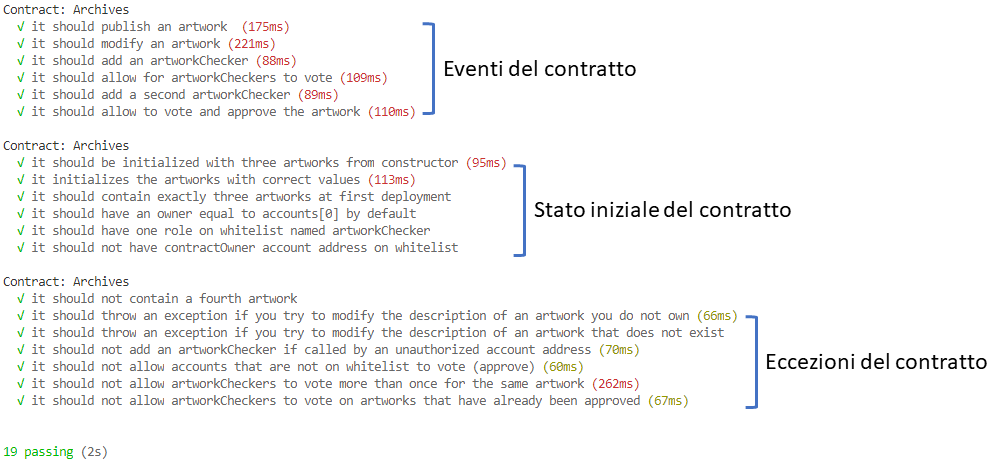
\includegraphics[width=1\textwidth]{immagini/testContratti.png}
\caption{Progetto: Risultato esecuzione dei test}
\label{fig:contractTests}
\end{figure}

\subsection{Applicazione client-side}

Ultimo passaggio della prima fase di sviluppo\footnote{Il processo di sviluppo del prototipo può essere consultato in questa repository, https://github.com/lukasd2/DigitalArchivesPrototype} consiste nella programmazione di un'interfaccia client-side da collegare con i contratti testati.

Web3.js è una collezione di librerie che permettono di effettuare operazioni di lettura e scrittura sulla blockchain, così come avviene ad esempio con \emph{Ajax} e i web server tradizionali. Fondamentalmente, a parte l’utilizzo di web3, il lato della programmazione front-end non subisce altri cambiamenti. Per le istruzioni di chiamata alla blockchain bisogna tenere conto dell’utilizzo delle funzioni asincrone e quindi gestire l’interfaccia e il flusso delle funzioni in modo adeguato per l’utente finale e per la gestione dei risultati in arrivo.

Per questo progetto si è scelto di costruire un'interfaccia minima con Bootstrap\footfullcite{bootstrap}, in figura \ref{fig:Prototipo} si vede la parte relativa all'inserimento di un oggetto nella blockchain. 

\begin{figure}[H]
\centering
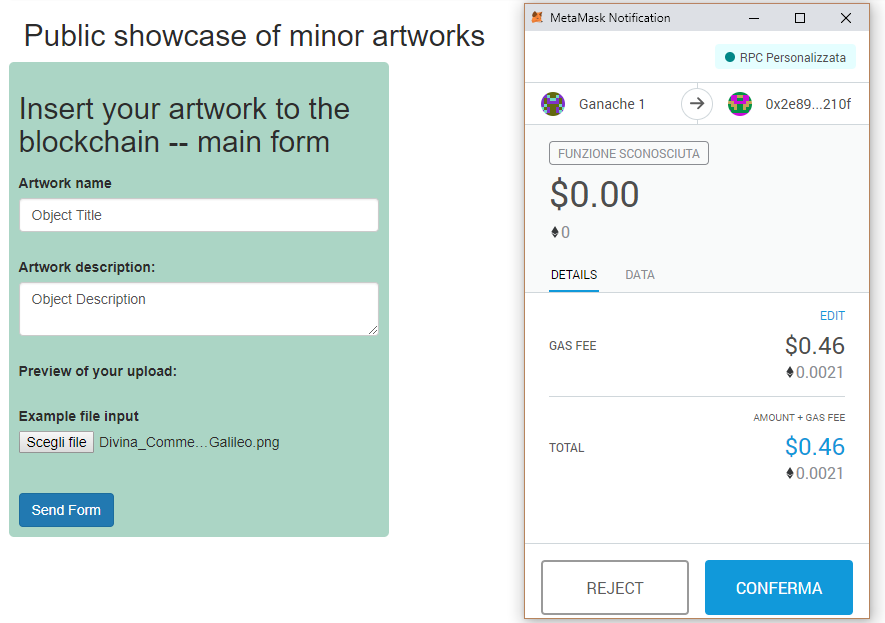
\includegraphics[width=1\textwidth]{immagini/prototype.PNG}
\caption{Progetto: Prototipazione inserimento oggetto sulla blockchain}
\label{fig:Prototipo}
\end{figure}

A questo punto è possibile testare il funzionamento della dApp attraverso l'interfaccia grafica. Per quanto riguarda le transazioni, ovvero le chiamate ai contratti che richiedono lo svolgimento di calcoli computazionali da parte della EVM, esse saranno intercettate da Metamask. In questa fase potrebbe essere utile passare da una blockchain con un funzionamento semplificato, impostando un nodo blockchain (privato) vero e proprio con Geth per accertarsi del funzionamento corretto della dApp.

\subsection{Integrazione con IPFS}

Nelle dApp che richiedono la memorizzazione di una quantità rilevante di dati, che nelle blockchain è tra le operazioni più costose, diventa indispensabile integrare un servizio di storage esterno. In questo progetto si utilizza IPFS per memorizzare e richiamare i dati troppo grandi per essere mantenuti direttamente su Ethereum. La figura \ref{fig:dapp} rappresenta l'impostazione finale della logica dell’applicazione.

\begin{figure}[H]
\centering
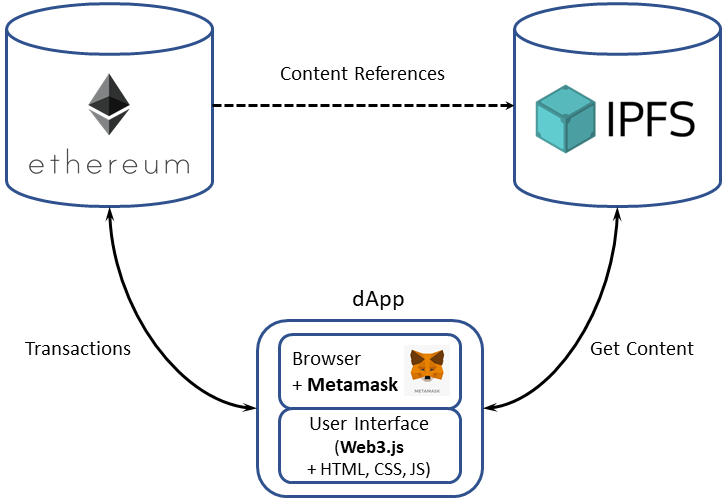
\includegraphics[width=1\textwidth]{immagini/ipfsIntegration.png}
\caption{Progetto: Logica dell'applicazione finale}
\label{fig:dapp}
\end{figure}

Seguendo questa impostazione la compilazione del modulo per l’inserimento di un nuovo oggetto include la spedizione delle risorse su IPFS. Prima di poter spedire la transazione sulla blockchain, la richiesta viene processata e rimane in attesa di upload sul servizio di storage. Se il caricamento avviene con successo, verrà restituito un indirizzo hash contenente i file caricati. A questo punto sarà possibile memorizzare il riferimento all'indirizzo IPFS sulla blockchain con una transazione. Ricapitolando, l'oggetto, la cui struttura è definita nel contratto, conterrà un puntatore all'indirizzo IPFS contenente la sua descrizione.
\\
\begin{lstlisting}[caption={Riferimento all'indirizzo hash di IPFS},language=JavaScript]
struct Artwork {
    ...
    string descriptionHash; //hash della descrizione dell'oggetto 
}
\end{lstlisting}

In questo modo si sfrutta la caratteristica di IPFS dell'indirizzamento basato sul contenuto, per cui è matematicamente certo che sotto un indirizzo hash sarà possibile trovare un dato dal contenuto immutabile, e con il progredire della tecnologia, permanente. Riguardo alla permanenza, il sistema IPFS allo stato dell'arte non ha implementato un meccanismo di incentivi, per cui, in questa applicazione, la memorizzazione viene effettuata attraverso Infura\footfullcite{infura}, una API che agisce da intermediario, in modo da mantenere il contenuto accessibile senza bisogno di mantenere un nodo personale (IPFS) costantemente attivo. Dunque una chiamata generica di caricamento del contenuto su IPFS avrà la seguente struttura:
\\
\begin{lstlisting}[caption={Aggiunta di file con IPFS Javascript API},language=JavaScript]
ipfs.files.add(data, [options], [callback])
\end{lstlisting}

Una delle principali funzionalità dell'applicazione, l'inserimento dell'oggetto sulla blockchain, è composta dalla seguente catena di operazioni:

\begin{enumerate}
    \item L'utente compila il modulo descrittivo dell'oggetto e preme il pulsante "Inserisci Oggetto"
    \item Il programma cattura i file (in questa implementazione immagini) rappresentative dell'oggetto e attraverso un Buffer\footnote{https://www.npmjs.com/package/buffer} li trasforma in una sequenza di dati binari
    \item La sequenza di bit viene caricata su IPFS
    \item IPFS ritorna un indirizzo hash per ciascuno dei file caricati che vengono memorizzati nella sessione in esecuzione del programma
    \item Il programma costruisce una descrizione completa dell'oggetto utilizzando la versione del sistema di metadati scelta dall'utente e include gli indirizzi hash dei file caricati. Con un’altra operazione di caricamento su IPFS il tutto viene raggruppato sotto un unico indirizzo hash che viene restituito al programma in esecuzione
    \item Il riferimento hash adesso può essere spedito e memorizzato sulla blockchain con una transazione effettuata e confermata dall'utente attraverso Metamask
    \item La descrizione completa dell'oggetto viene richiamata utilizzando il riferimento memorizzato sulla blockchain che punta alla posizione contenuta su IPFS
\end{enumerate}


\subsection{Costruzione dell'interfaccia finale}

Una volta implementata la logica completa dell’applicazione, seguita da una fase di test per verificarne la correttezza, è stata costruita l’interfaccia grafica finale. Per questa fase di programmazione \emph{front-end} si è scelto di utilizzare Bulma\footfullcite{bulma} e Sass\footfullcite{sass}. Bulma è un framework CSS basato su \emph{flexbox} con un certo numero di elementi grafici predefiniti e un sistema di griglia che facilita la costruzione di layout flessibili, mentre Sass è un preprocessore CSS, serve principalmente per velocizzare e rendere più efficiente lo sviluppo dei fogli di stile\footnote{Sass estende i fogli di stile con diverse funzionalità tra cui la possibilità di utilizzare variabili, funzioni modulari (mixins), operazioni matematiche ecc.}. In figura \ref{fig:indexApp} è possibile vedere la pagina iniziale dell'applicazione.

\begin{figure}[H]
\centering
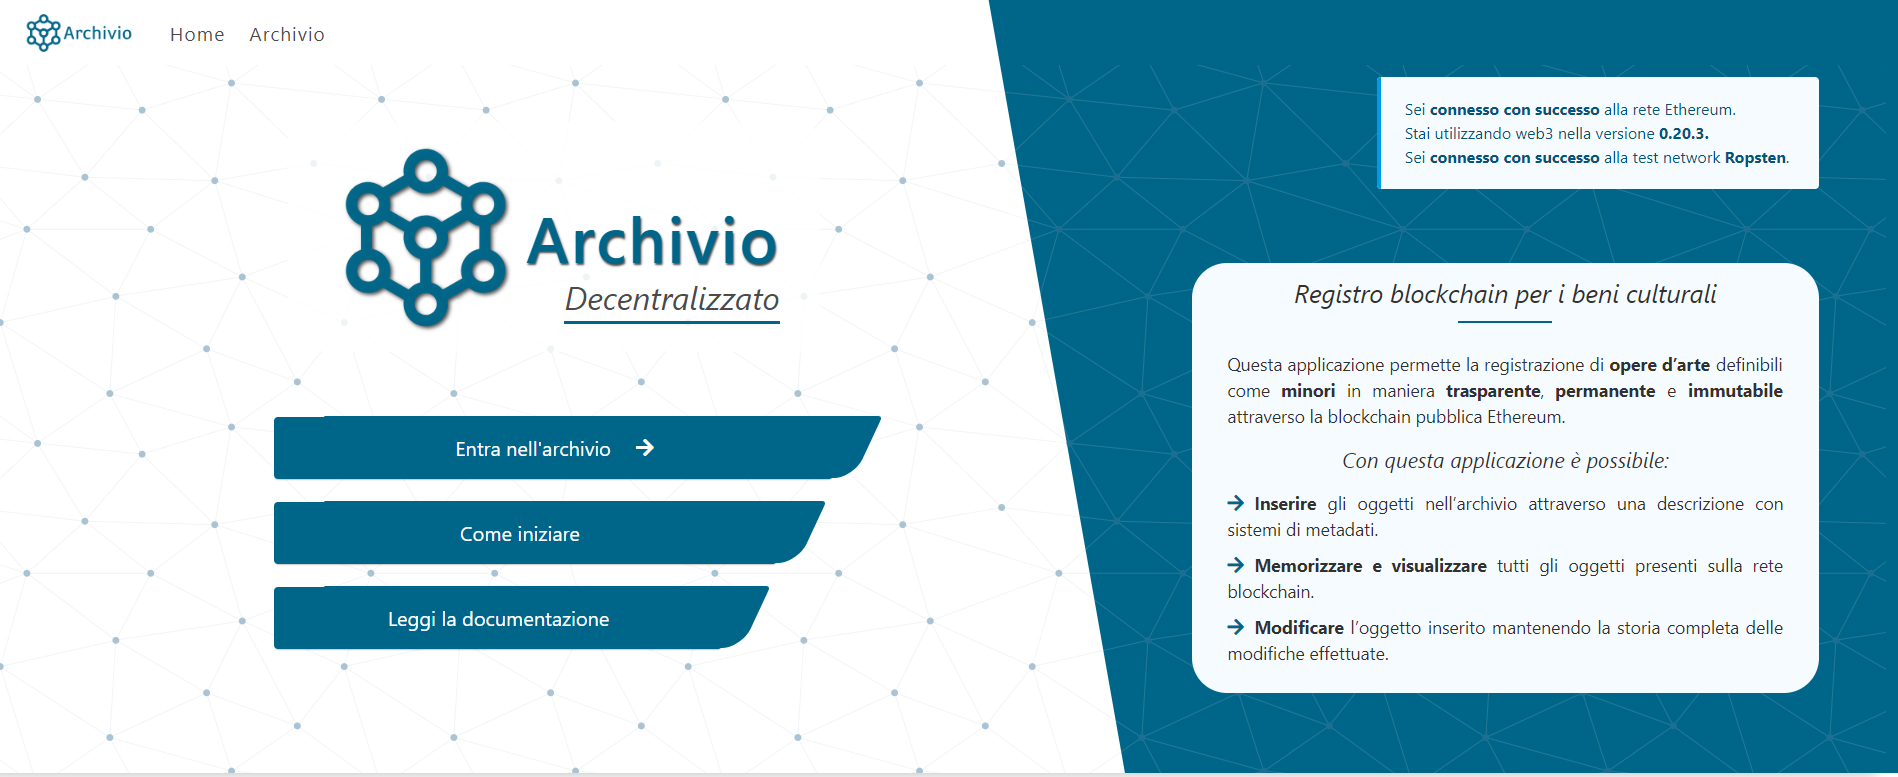
\includegraphics[width=1\textwidth]{immagini/prova3Index.PNG}
\caption{Progetto: Pagina iniziale dell'applicazione}
\label{fig:indexApp}
\end{figure}

Questa pagina serve a dare informazioni essenziali sulle funzionalità del progetto e i vantaggi derivanti dall'utilizzo della blockchain. Inoltre serve da guida per l'utilizzo delle dApps e si ricollega direttamente ai contenuti di questo elaborato.

La parte principale dell'applicazione, contente l'archivio, è illustrata in figura \ref{fig:artworkApp}.

\begin{figure}[H]
\centering
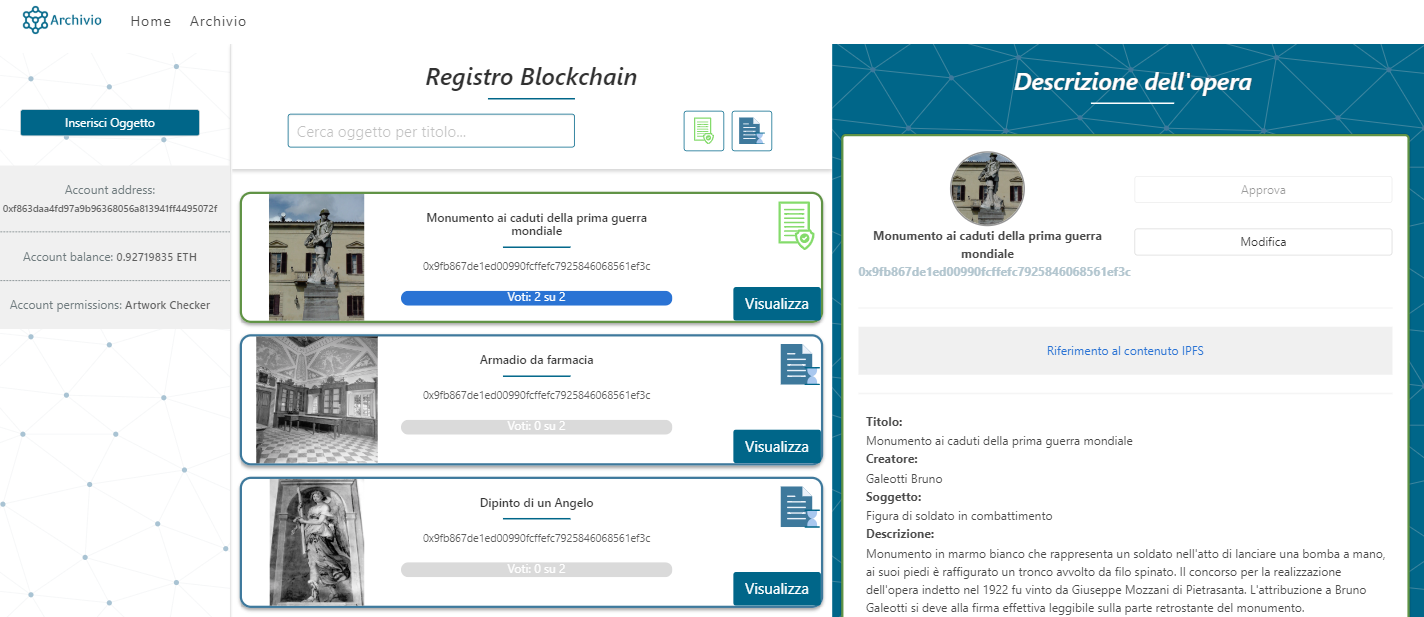
\includegraphics[width=1\textwidth]{immagini/artwork3Prova.PNG}
\caption{Progetto: Pagina contente l'archivio blockchain}
\label{fig:artworkApp}
\end{figure}

Con questa impostazione dell'interfaccia finale l'applicazione è divisa logicamente, da sinistra verso destra, in tre parti. Nella parte sinistra è possibile attivare il modulo per l'inserimento di un oggetto nel registro e consultare le informazioni principali relative al proprio account (l'indirizzo utente, il bilancio di token e i permessi). 

La parte centrale contiene l'archivio di tutte le opere registrate sulla blockchain e le informazioni principali relative a ciascun oggetto come illustrato di seguito nella figura \ref{fig:artworkFocus}. Inoltre permette di "filtrare" gli oggetti in base al loro stato di approvazione e di effettuare una ricerca per titolo tramite un input situato in alto a sinistra.

La parte a destra contiene la descrizione completa di ciascun oggetto inserito nell'archivio. In particolare i metadati e le immagini descrittive vengono richiamate da IPFS attraverso l'indirizzo hash memorizzato direttamente sulla blockchain. Una volta selezionato l'oggetto dell'archivio tramite il pulsante "visualizza", queste informazioni saranno raggruppate e compariranno in questa sezione del sito. 

\begin{figure}[H]
\centering
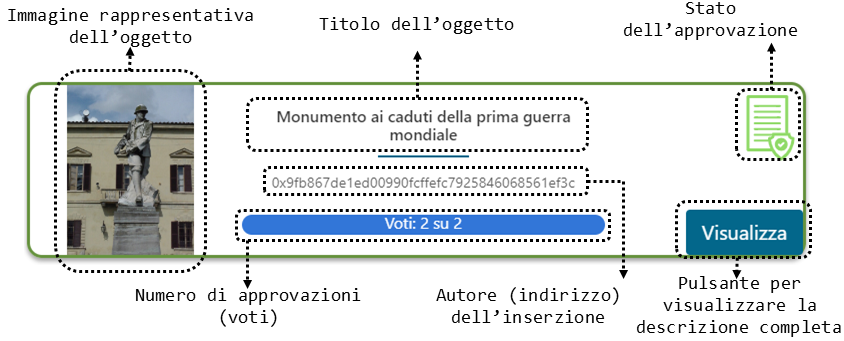
\includegraphics[width=1\textwidth]{immagini/artworkFocusCommented.png}
\caption{Progetto: Archivio la scheda di un oggetto}
\label{fig:artworkFocus}
\end{figure}

\subsection{Ethereum Testnet}

Il trasferimento dei contratti su una blockchain Ethereum di prova (\emph{testnet}) conclude lo sviluppo di questo progetto. Ethereum ha diverse reti di sviluppo, comunemente chiamate testnet, utili allo scopo di provare il funzionamento dei contratti prima di farne il deploy sulla rete principale. 

La differenza fondamentale tra queste reti e la rete principale (\emph{mainnet}) deriva dall’utilizzo di token che non hanno un valore reale al di fuori dell'ambiente di prova, dunque è possibile creare le proprie applicazioni e pubblicarle eseguendo dei test sulla determinata blockchain di sviluppo evitando di dover sostenere spese legate alle transazioni.

In questo progetto si è scelto di pubblicare i contratti su Ropsten\footfullcite{ropsten}, una blockchain di prova che, al momento dello scrivere, utilizza lo stesso sistema di consenso (Proof of Work) della rete principale. È una rete in grado di riprodurre con un buon grado di precisione il funzionamento di mainnet, questo è particolarmente utile per verificare le stime relative ai costi delle transazioni e tutti gli aspetti legati al funzionamento della dApp stessa. Questa fase risulta fondamentale nel processo di sviluppo di un’applicazione decentralizzata ed è raccomandabile effettuarla con un numero di utenti il più ampio possibile per raccogliere i dati (\emph{feedback}) circa il funzionamento di smart contracts e delle dApps in modo da trovare eventuali errori prima di pubblicare l'applicazione sulla blockchain principale.
\chapter{Conclusioni}

\printbibliography

\end{document}